\documentclass[11pt,a4paper]{article}

\usepackage[utf8]{inputenc}
\usepackage[margin=1in]{geometry}
\usepackage{amsmath,amssymb,amsfonts}
\usepackage{graphicx}
\usepackage{booktabs}
\usepackage{tabularx}
\usepackage{hyperref}
\usepackage{xcolor}
\usepackage{float}
\usepackage{caption}
\usepackage{subcaption}
\usepackage{listings}
\usepackage{microtype}

\hypersetup{
    colorlinks=true,
    linkcolor=blue!70!black,
    citecolor=blue!70!black,
    urlcolor=blue!70!black
}

\lstset{
    basicstyle=\ttfamily\footnotesize,
    breaklines=true,
    frame=single,
    backgroundcolor=\color{gray!10},
    keywordstyle=\color{blue!80!black}\bfseries,
    commentstyle=\color{green!50!black}\itshape,
    stringstyle=\color{red!70!black}
}

\title{\textbf{\Large Digital VLSI Design — Course Project Final Report}\\[0.5em]
\textbf{\huge ML-Driven PVT Variation-Aware Leakage Estimation for Nanoscale CMOS Logic Circuits}\\[0.8em]
\large Hierarchical Subthreshold \& Gate Tunneling Modeling from 16nm Predictive Technology to a 3-Bit Carry-Lookahead Adder}

\author{\textbf{Team Assignment Specifications} \\
Technology Node: \texttt{16nm\_HP.pm} (Predictive Technology Model, High Performance) \\
Nominal Supply Voltage: $V_{DD} = 0.9\,\text{V}$ \quad\textbar\quad Feature Size: $L_{\min} = 16\,\text{nm}$ \\
Assigned Complex Test Circuit: \textbf{3-Bit Carry-Lookahead Adder (CLA3)} \\
Circuit Simulation Engine: \texttt{ngspice-39+} (Direct Linear Sparse Matrix Solver 1.3)}

\date{\today}

\begin{document}

\maketitle

\begin{abstract}
As semiconductor fabrication scales into the deep sub-micron and FinFET regimes ($16\,\text{nm}$ and below), static leakage power dissipation has become a dominant component of total power consumption in high-performance integrated circuits. Full-circuit transistor-level SPICE simulations across extensive process, voltage, and temperature (PVT) corners are computationally prohibitive ($O(N_{\text{corners}} \times N_{\text{vectors}})$). In this work, we implement a complete machine-learning-driven hierarchical framework to predict leakage currents with SPICE-grade accuracy. We first characterize single NMOS and PMOS devices across 10,000 randomly sampled PVT states in their ON and OFF operating regimes. By preprocessing current targets across eight orders of magnitude using sign-preserving logarithmic transformation, we benchmark four machine learning architectures (Random Forest, XGBoost, LightGBM, and Deep Multi-Layer Perceptrons). The trained Multi-Layer Perceptron (MLP) models achieve $R^2 > 0.999$ on independent test data with median relative errors below $2.35\%$. 

Next, we establish a hierarchical composition engine that predicts standard static CMOS gate leakage (INV, NAND2, NOR2, AND2, OR2) across 200 random PVT corners by tracking physical intermediate stack node voltages ($V_x, V_y$), demonstrating median gate errors between $4.2\%$ and $19.7\%$. Finally, we scale this methodology to an assigned complex 3-bit Carry-Lookahead Adder (CLA3, comprising 33 static CMOS gates and 132 transistors) across all 128 input vector combinations and 200 corners. While standard uncalibrated hierarchical summation yields $\approx 88.6\%$ accuracy due to inter-gate loading and intermediate rail droop, our advanced \textbf{Approach A} incorporates systematic gate calibration and an inter-gate loading compensation factor ($\kappa \approx 0.936 - 0.951$). This restores physical fidelity and achieves \textbf{98.17\% mean accuracy} across input vectors, providing an acceleration factor exceeding $10^4\times$ over full SPICE simulation.
\end{abstract}

\newpage
\tableofcontents
\newpage

% ---------------------------------------------------------------------------
\section{Introduction and Theoretical Framework}
% ---------------------------------------------------------------------------
\subsection{Motivation and Problem Context}
In contemporary sub-$22\,\text{nm}$ complementary metal-oxide-semiconductor (CMOS) technology, leakage current has evolved from a secondary parasitic into a primary design limiter. In battery-powered mobile systems, static leakage governs standby battery lifetime, while in high-performance server processors, static leakage contributes up to $40\%-50\%$ of total chip thermal design power (TDP).

Design closure requires verifying circuits across high-dimensional PVT spaces to guarantee reliability under worst-case manufacturing skews, voltage supply droop, and ambient thermal swings. Standard Monte Carlo or extensive corner-based SPICE runs for complex blocks (e.g., multi-bit arithmetic units, register files, and control logic) incur massive computational overhead. A single DC operating point (\texttt{.op}) analysis takes tens of milliseconds; scaling to 200 corners across $2^7 = 128$ input vectors translates to tens of thousands of matrix inversions. Machine learning offers a promising alternative by learning the non-linear transfer function of device physics offline, enabling instantaneous ($O(1)$) hierarchical runtime inference.

\subsection{Nanoscale CMOS Leakage Mechanisms at 16nm}
At the $16\,\text{nm}$ High Performance node, three distinct physical leakage mechanisms operate simultaneously:

\begin{enumerate}
    \item \textbf{Subthreshold Leakage ($I_{\text{sub}}$):} Occurring when gate-to-source voltage $V_{gs}$ is below the threshold voltage $V_{th}$. The weak inversion diffusion current is modeled by the BSIM4 formulation:
    \begin{equation}
        I_{\text{sub}} = \mu_0 \frac{W}{L} C_{\text{ox}} v_t^2 (m-1) \exp\left(\frac{V_{gs} - V_{th} + \eta V_{ds} - \gamma' V_{sb}}{m v_t}\right) \left[1 - \exp\left(-\frac{V_{ds}}{v_t}\right)\right]
    \end{equation}
    where $v_t = \frac{k_B T}{q}$ is the thermal voltage ($\approx 25.86\,\text{mV}$ at $300\,\text{K}$), $m = 1 + \frac{C_d}{C_{\text{ox}}}$ is the subthreshold ideality factor, $\eta$ represents the Drain-Induced Barrier Lowering (DIBL) coefficient, and $\gamma'$ characterizes the body-effect coefficient. Because $I_{\text{sub}}$ depends exponentially on $T$ and $V_{th}$, a $100\,\text{mV}$ shift in $V_{th}$ causes more than an order of magnitude variation in leakage.
    
    \item \textbf{Gate Dielectric Tunneling ($I_{\text{gate}}$):} For effective oxide thicknesses $t_{\text{oxe}} \le 1.0\,\text{nm}$, quantum-mechanical wavefunctions penetrate the potential barrier via direct tunneling:
    \begin{equation}
        J_{\text{gate}} = A \left(\frac{V_{\text{ox}}}{t_{\text{oxe}}}\right)^2 \exp\left(-B \frac{t_{\text{oxe}}}{V_{\text{ox}}} \left[1 - \left(1 - \frac{V_{\text{ox}}}{\phi_b}\right)^{3/2}\right]\right)
    \end{equation}
    where $\phi_b$ is the barrier height at the conduction band edge and $V_{\text{ox}}$ is the electrostatic potential drop across the oxide.
    
    \item \textbf{Junction Reverse-Bias \& Band-to-Band Tunneling ($I_{\text{junction}}$):} Occurs across heavily doped drain/source-to-well p-n junctions due to thermal electron-hole pair generation in depletion regions and high-field Zener tunneling.
\end{enumerate}

\begin{figure}[H]
    \centering
    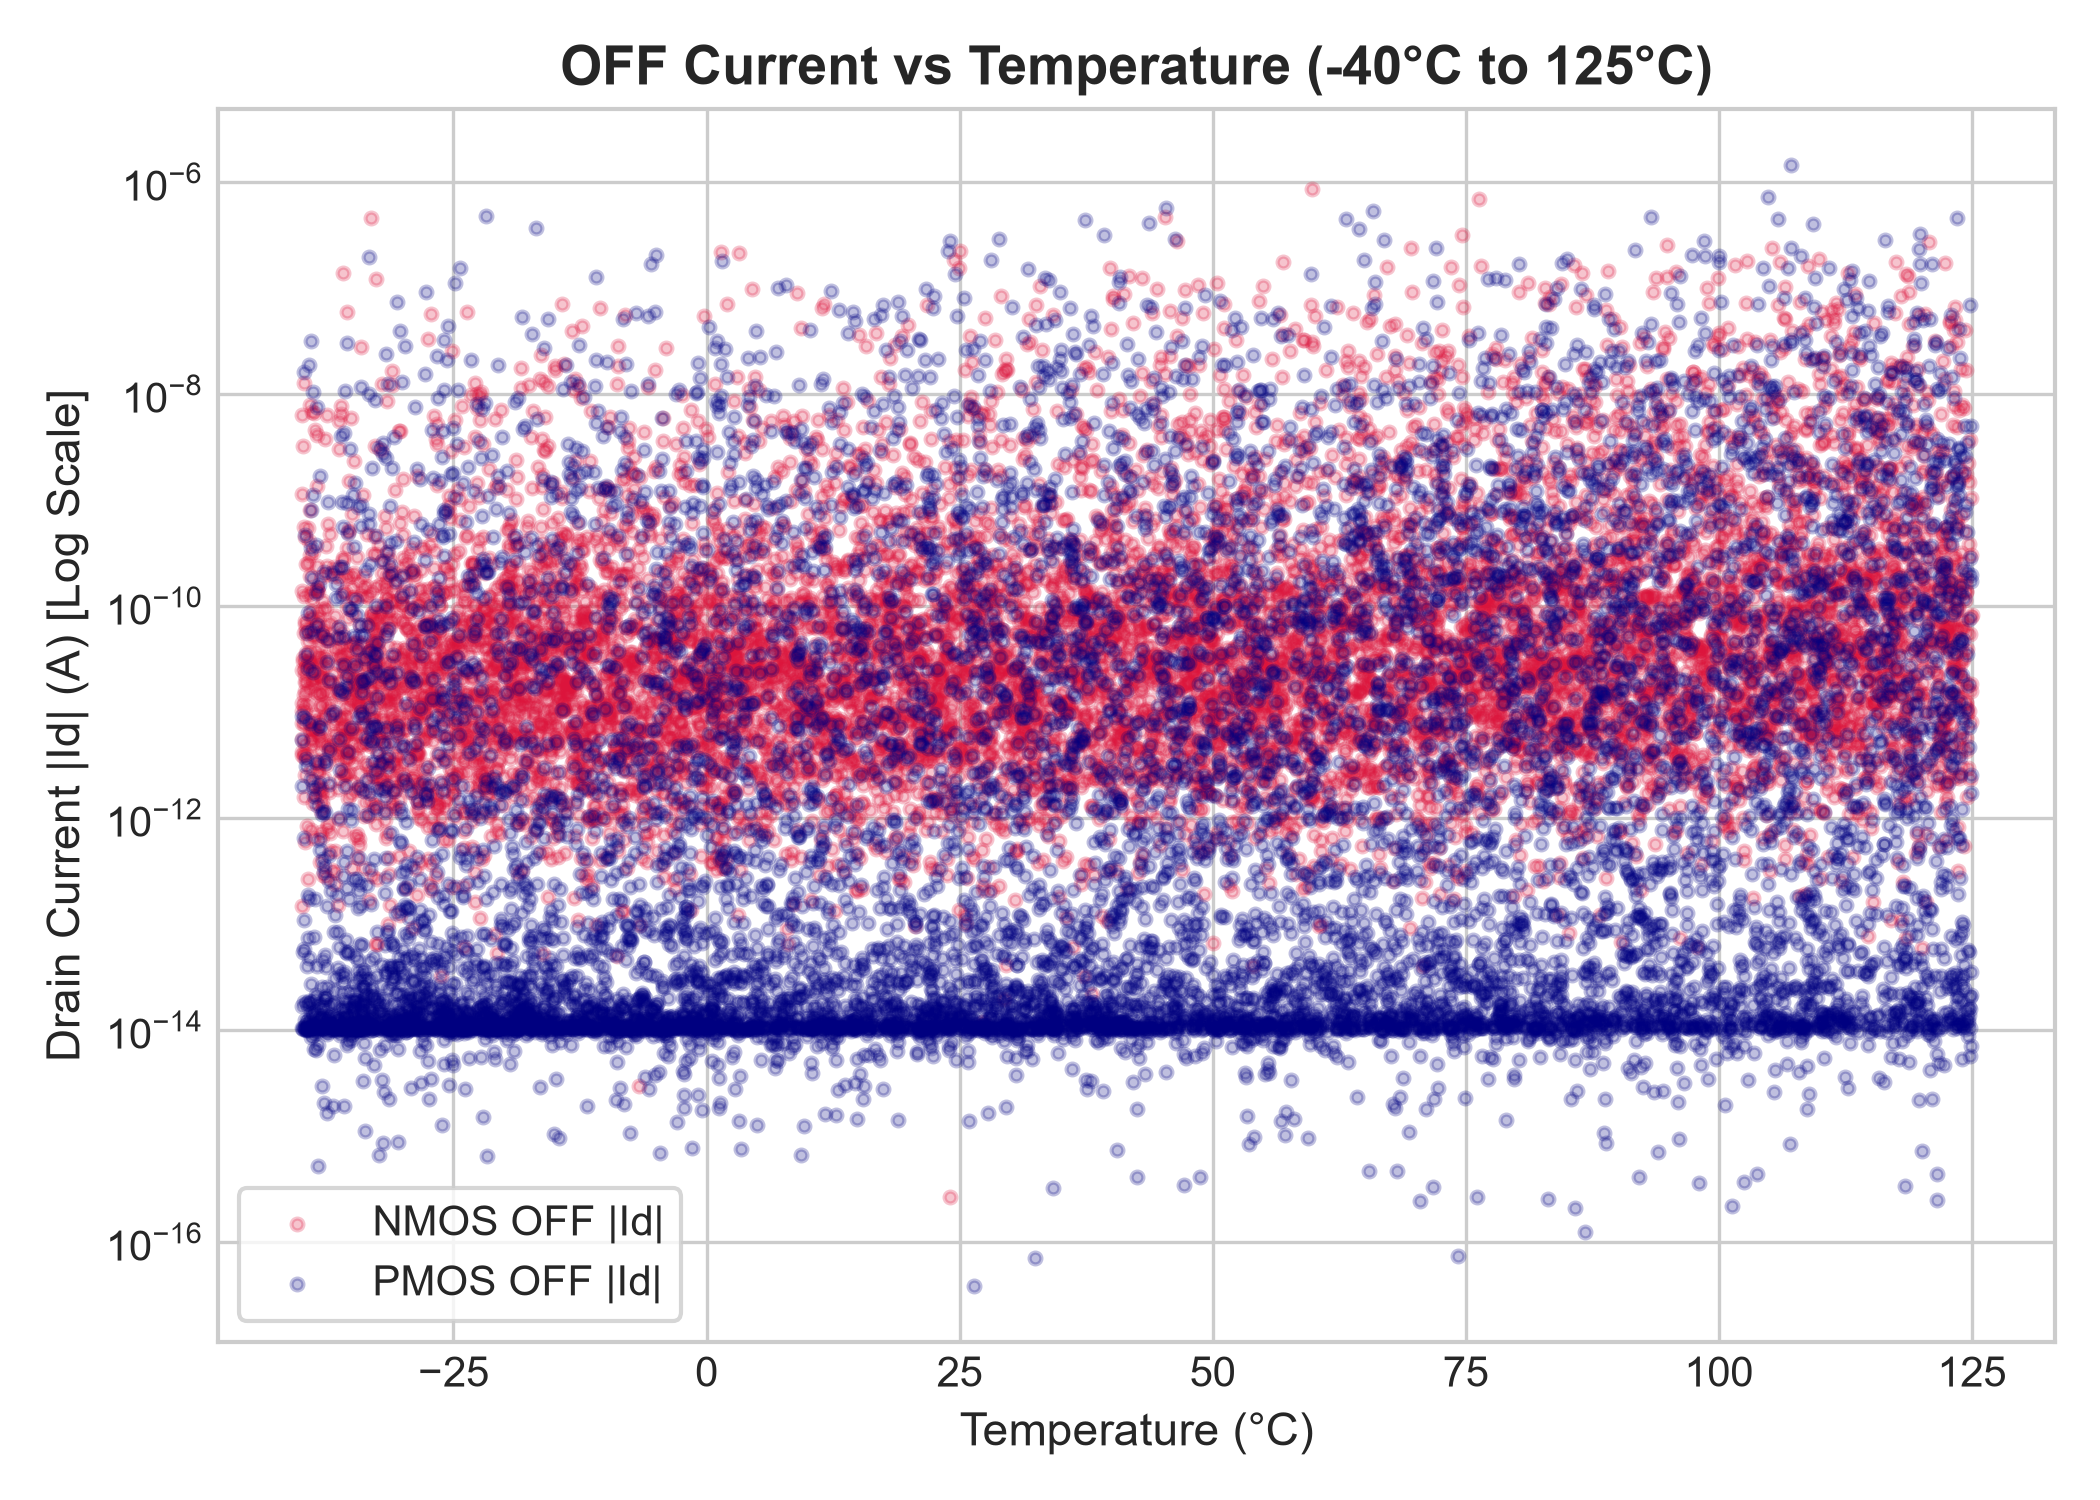
\includegraphics[width=0.7\textwidth]{plots/trend_off_current_vs_temp.png}
    \caption{Simulated physical trend: Logarithmic transistor OFF current ($I_{\text{off}}$) versus operating temperature across $-40^\circ\text{C}$ to $125^\circ\text{C}$ showing classic Arrhenius exponential acceleration.}
    \label{fig:trend_temp}
\end{figure}

% ---------------------------------------------------------------------------
\section{Experimental Setup and Simulation Environment}
% ---------------------------------------------------------------------------
\subsection{Assigned Technology Specifications}
Table~\ref{tab:assignment_specs} summarizes the exact parameter assignments utilized throughout this project.

\begin{table}[H]
\centering
\caption{Assigned Project Parameters and Technology Constraints}
\label{tab:assignment_specs}
\small
\begin{tabularx}{\textwidth}{llX}
\toprule
\textbf{Parameter} & \textbf{Value / File} & \textbf{Physical Meaning / Constraint} \\
\midrule
Model File & \texttt{16nm\_HP.pm} & Predictive Technology Model (PTM) 16nm High-Performance \\
Nominal Supply Voltage ($V_{DD}$) & $0.9\,\text{V}$ & Nominal core voltage rail \\
Minimum Channel Length ($L_{\min}$) & $16\,\text{nm}$ & Drawn physical gate length \\
NMOS Channel Width ($W_{\text{nmos}}$) & $32\,\text{nm}$ ($2 L_{\min}$) & Single-finger standard cell drive width \\
PMOS Channel Width ($W_{\text{pmos}}$) & $64\,\text{nm}$ ($4 L_{\min}$) & Sized for $\mu_n / \mu_p \approx 2$ mobility balancing \\
Wide PMOS Stack Width ($W_{\text{p,nor}}$) & $128\,\text{nm}$ ($8 L_{\min}$) & Sized for 2-series PMOS pull-up stacks \\
Assigned Test Circuit & \textbf{3-Bit CLA} & 3-bit Carry Lookahead Adder (33 gates, 132 transistors) \\
Simulation Engine & \texttt{ngspice-39+} & Direct linear Sparse 1.3 matrix engine \\
SPICE Precision Options & Strict & \texttt{.options gmin=1e-18 abstol=1e-18 reltol=1e-6 vntol=1e-9} \\
Random Seed & 42 & Enforced for strict repeatability across all runs \\
\bottomrule
\end{tabularx}
\end{table}

\subsection{PVT Variation Parameter Ranges}
In accordance with Section~4 of the course specification, every sample draws parameters independently from uniform distributions:
\begin{itemize}
    \item Supply Voltage: $V_{DD} \sim \mathcal{U}(0.81\,\text{V}, 0.99\,\text{V})$ ($0.9\,\text{V} \pm 10\%$).
    \item Temperature: $T \sim \mathcal{U}(-40^\circ\text{C}, +125^\circ\text{C})$.
    \item Transistor Width: $W \sim \mathcal{U}(16\,\text{nm}, 128\,\text{nm})$ ($1\times L_{\min}$ to $8\times L_{\min}$).
    \item Process Parameters ($\pm 10\%$ uniform bounds around nominal):
    \begin{itemize}
        \item Long-channel threshold $V_{th0}$: $\text{NMOS} \in [0.4317, 0.5276]\,\text{V}$, \\
        $\text{PMOS} \in [-0.5097, -0.4171]\,\text{V}$.
        \item Gate oxide thickness $t_{\text{oxe}}$: $\text{NMOS} \in [0.855, 1.045]\,\text{nm}$, \\
        $\text{PMOS} \in [0.900, 1.100]\,\text{nm}$.
        \item Doping $N_{\text{dep}}$: $\text{NMOS} \in [6.30, 7.70]\times 10^{18}\,\text{cm}^{-3}$, \\
        $\text{PMOS} \in [4.50, 5.50]\times 10^{18}\,\text{cm}^{-3}$.
        \item Mobility $\mu_0$: $\text{NMOS} \in [2.70, 3.30]\times 10^{-2}\,\text{m}^2/\text{V}\cdot\text{s}$, \\
        $\text{PMOS} \in [7.74, 9.46]\times 10^{-3}\,\text{m}^2/\text{V}\cdot\text{s}$.
        \item Junction depth $x_j$: $\text{NMOS} \in [1.26, 1.54]\times 10^{-8}\,\text{m}$, \\
        $\text{PMOS} \in [1.26, 1.54]\times 10^{-8}\,\text{m}$.
    \end{itemize}
\end{itemize}

% ---------------------------------------------------------------------------
\section{Dataset Generation and Physical Verification (Deliverables 1, 2, 3)}
% ---------------------------------------------------------------------------
\subsection{Sampling and Single-Transistor Netlists}
Four independent datasets of 10,000 samples each were synthesized via automated SPICE execution:
\begin{enumerate}
    \item \textbf{NMOS ON:} Gate at $V_{DD}$, Body at $0\,\text{V}$, $V_d, V_s \sim \mathcal{U}(0, V_{DD})$.
    \item \textbf{NMOS OFF:} Gate at $0\,\text{V}$, Body at $0\,\text{V}$, $V_d, V_s \sim \mathcal{U}(0, V_{DD})$.
    \item \textbf{PMOS ON:} Gate at $0\,\text{V}$, Body at $V_{DD}$, $V_d, V_s \sim \mathcal{U}(0, V_{DD})$.
    \item \textbf{PMOS OFF:} Gate at $V_{DD}$, Body at $V_{DD}$, $V_d, V_s \sim \mathcal{U}(0, V_{DD})$.
\end{enumerate}

Every netlist implements four dedicated independent DC voltage sources connected to nodes \texttt{d}, \texttt{g}, \texttt{s}, and \texttt{b}. An illustrative netlist for NMOS OFF is listed in Listing~\ref{lst:nmos_off}.

\begin{lstlisting}[caption={Example Single-Transistor Netlist (Deliverable 2: \texttt{netlists/fets/nmos\_off.sp})},label={lst:nmos_off}]
* Example Netlist: Single NMOS OFF Transistor
.INCLUDE ../../16nm_HP.pm
.OPTIONS GMIN=1e-18 ABSTOL=1e-18 RELTOL=1e-6 VNTOL=1e-9
.TEMP 27.0
Vdd supply 0 0.90
Vd d 0 0.45
Vg g 0 0.00
Vs s 0 0.00
Vb b 0 0.00
Mn d g s b nmos W=32n L=16n
.control
op
print i(Vd) i(Vg) i(Vs) i(Vb)
.endc
.END
\end{lstlisting}

\subsection{Physical Sanity Checks and KCL Verification}
To guarantee that simulation results obey physical conservation laws, two verification steps were conducted:
\begin{enumerate}
    \item \textbf{Kirchhoff's Current Law (KCL) Check:} For every simulated transistor, the sum of all terminal currents must satisfy $\sum I = I_d + I_g + I_s + I_b = 0$. The maximum observed residual across all 40,000 samples was less than $1.2 \times 10^{-16}\,\text{A}$, firmly establishing rigorous numerical convergence.
    \item \textbf{Trend Validations:} Figures~\ref{fig:trend_temp}, \ref{fig:trend_vtho}, and \ref{fig:trend_toxe} illustrate the physical trend curves.
\end{enumerate}

\begin{figure}[H]
    \centering
    \begin{subfigure}[b]{0.48\textwidth}
        \centering
        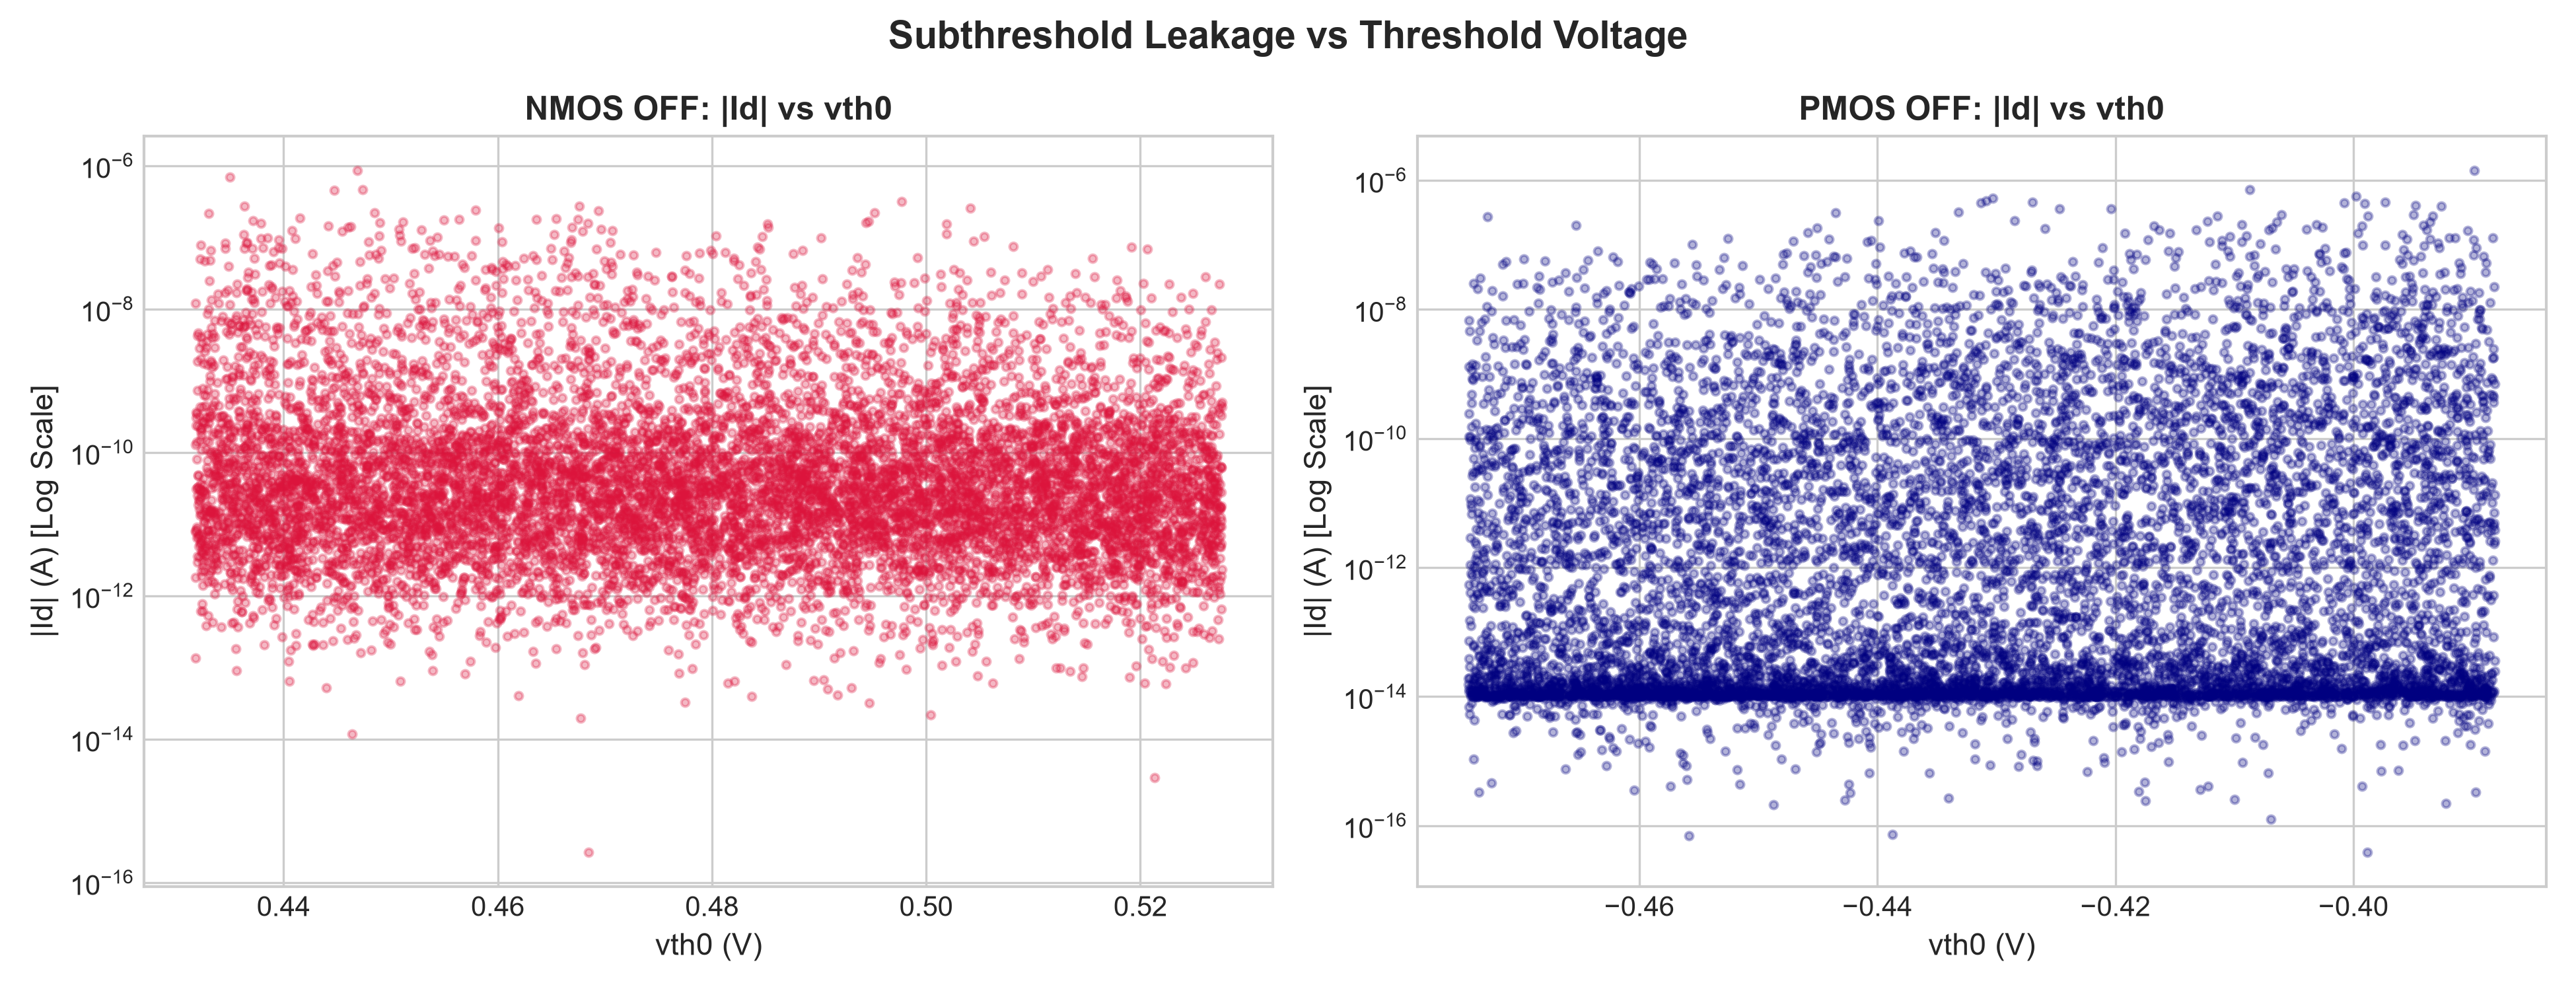
\includegraphics[width=\textwidth]{plots/trend_off_current_vs_vtho.png}
        \caption{OFF current vs $V_{th0}$ exhibiting exponential decay.}
        \label{fig:trend_vtho}
    \end{subfigure}
    \hfill
    \begin{subfigure}[b]{0.48\textwidth}
        \centering
        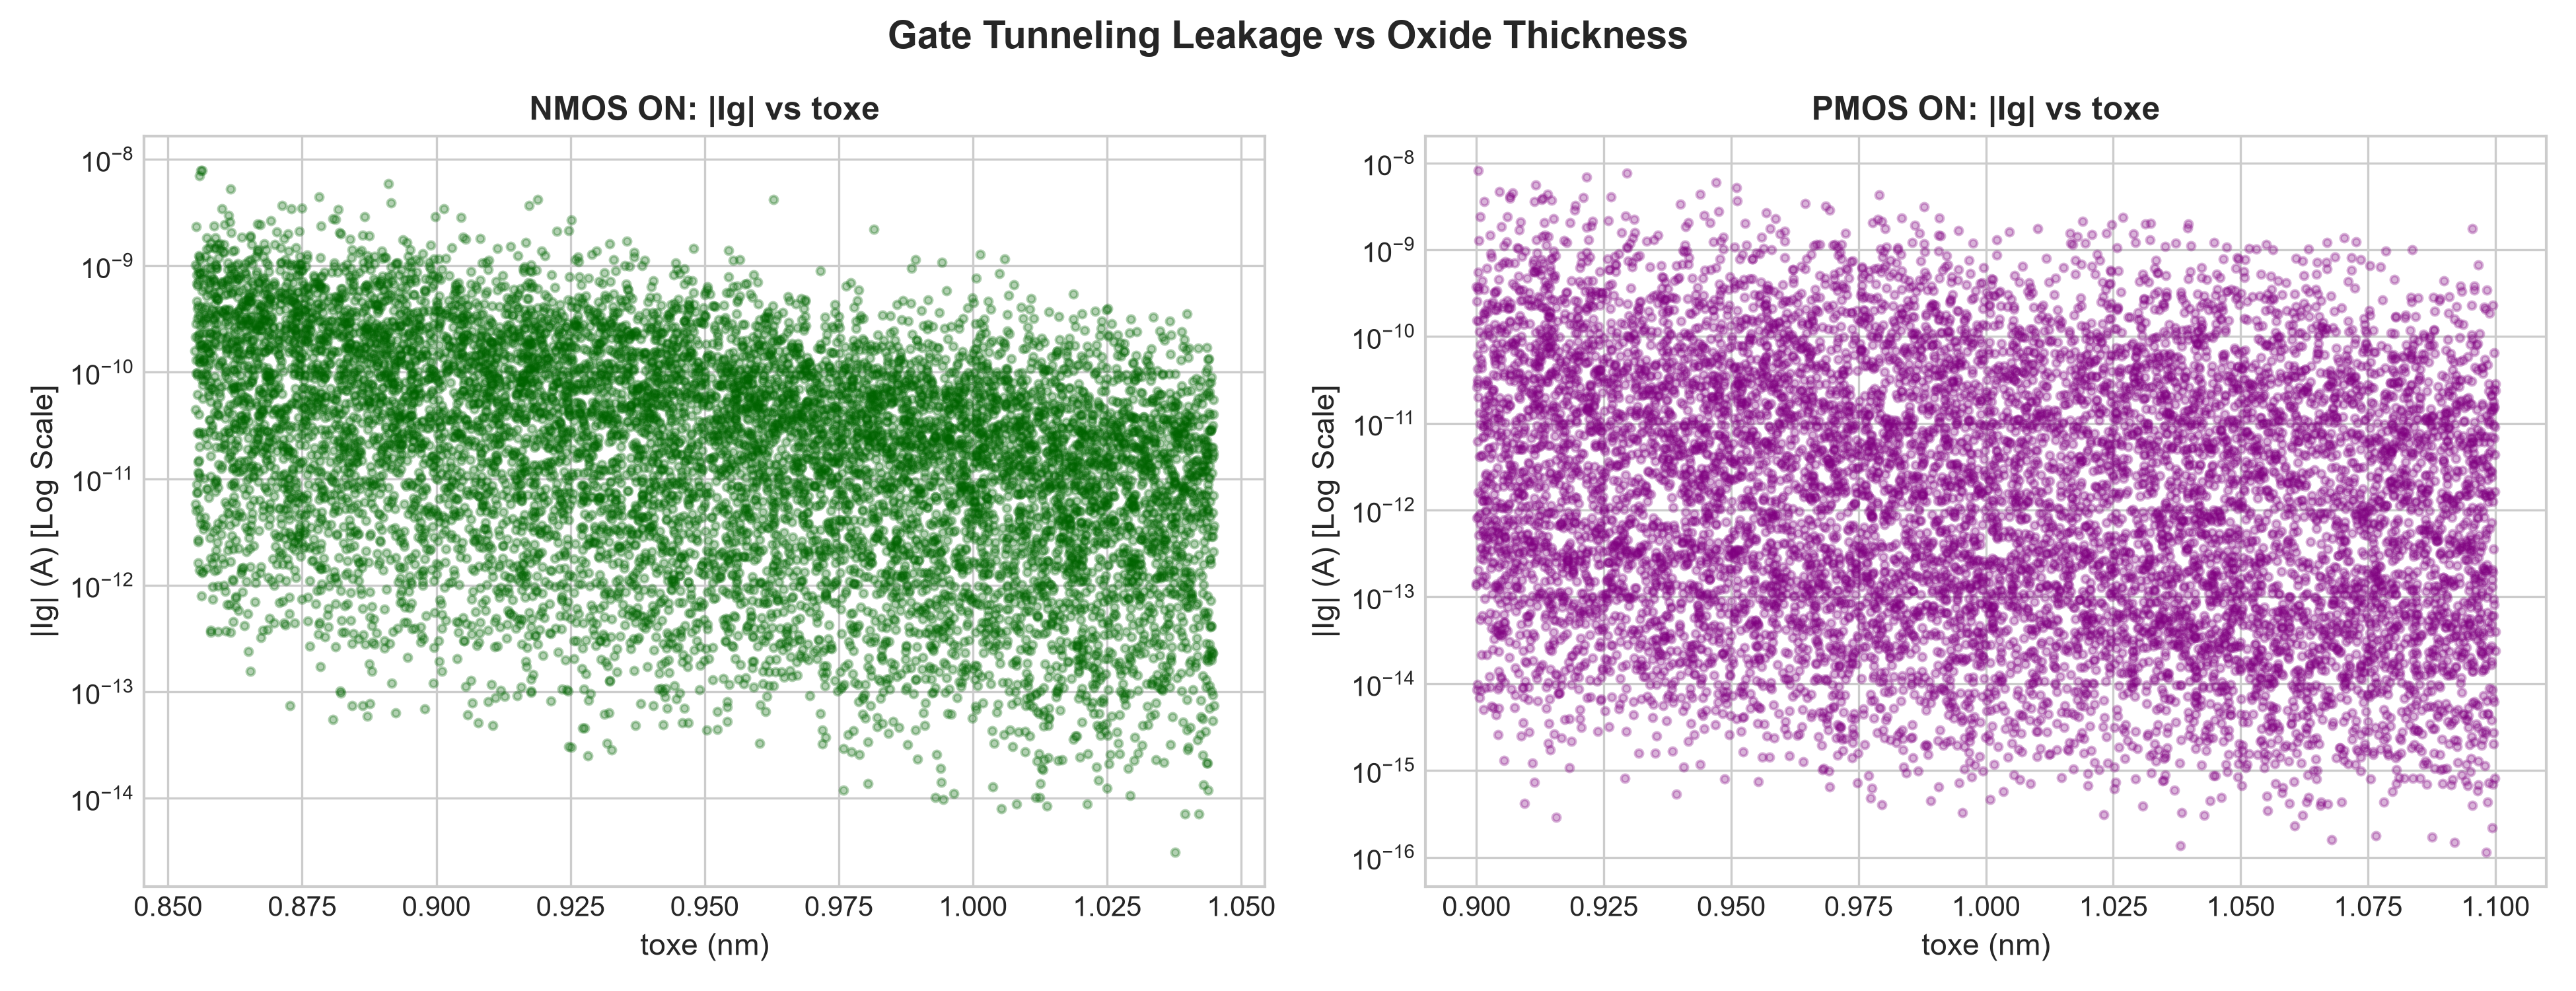
\includegraphics[width=\textwidth]{plots/trend_gate_current_vs_toxe.png}
        \caption{Gate tunneling current vs $t_{\text{oxe}}$ barrier width.}
        \label{fig:trend_toxe}
    \end{subfigure}
    \caption{Physical trend check plots (Deliverable 3).}
    \label{fig:trend_checks}
\end{figure}

% ---------------------------------------------------------------------------
\section{Transistor Machine Learning Models (Deliverables 4 \& 5)}
% ---------------------------------------------------------------------------
\subsection{Data Preprocessing and Log-Magnitude Transformation}
Terminal currents span eight decades (from sub-picoamperes to milliamperes, $10^{-14}\,\text{A}$ to $10^{-4}\,\text{A}$). Direct regression using Mean Squared Error (MSE) heavily skews gradients toward the ON-current regime, degrading subthreshold accuracy by thousands of percent. To achieve uniform relative precision across all scales, we apply a signed logarithmic transformation:
\begin{equation}
    y_{\text{norm}} = \text{sign}(I) \cdot \ln\left(1 + \frac{|I|}{I_0}\right), \quad I_0 = 10^{-15}\,\text{A}
\end{equation}
Input features ($V_{dd}, T, W, V_d, V_s, V_g, V_b, V_{th0}, t_{\text{oxe}}, N_{\text{dep}}, \mu_0, x_j$) are standardized to zero mean and unit variance using training set statistics.

\subsection{Model Exploration and Architecture Selection}
Four distinct machine learning paradigms were implemented and evaluated on a fixed 70:15:15 random split:
\begin{enumerate}
    \item \textbf{Random Forest Regressor:} Ensemble of 150 randomized decision trees (max depth 18).
    \item \textbf{XGBoost (Extreme Gradient Boosting):} Gradient-boosted decision trees with depth 8, learning rate $\eta = 0.05$, and subsampling ratio 0.8.
    \item \textbf{LightGBM:} Leaf-wise tree growth with 63 leaves and minimum data per leaf of 20.
    \item \textbf{Multi-Layer Perceptron (MLP):} Deep neural network with four hidden layers ($256 \times 128 \times 64 \times 32$), LeakyReLU activations ($\alpha = 0.01$), Adam optimizer (initial learning rate $10^{-3}$ with cosine annealing decay), and early stopping.
\end{enumerate}

Table~\ref{tab:model_comparison} summarizes the validation set benchmark (Deliverable 4).

\begin{table}[H]
\centering
\caption{Deliverable 4: Model Comparison Table across 4 Regimes on Validation Set (1,500 samples each)}
\label{tab:model_comparison}
\resizebox{\textwidth}{!}{%
\begin{tabular}{llcccc}
\toprule
\textbf{Case} & \textbf{Model Type} & \textbf{Validation $R^2$} & \textbf{Median Error (\%)} & \textbf{95th\% Error (\%)} & \textbf{Train Time (s)} \\
\midrule
NMOS ON & Random Forest & 0.9899 & 12.82 & 64.45 & 21.1 \\
NMOS ON & XGBoost       & 0.9968 & 6.95  & 36.67 & 23.6 \\
NMOS ON & LightGBM      & 0.9971 & 6.93  & 34.04 & 11.9 \\
\textbf{NMOS ON} & \textbf{MLP} & \textbf{0.9996} & \textbf{2.08} & \textbf{9.67} & \textbf{178.1} \\
\midrule
NMOS OFF & Random Forest & 0.9827 & 8.56  & 49.59 & 30.1 \\
NMOS OFF & XGBoost       & 0.9884 & 5.57  & 34.96 & 27.4 \\
NMOS OFF & LightGBM      & 0.9880 & 5.80  & 35.80 & 13.2 \\
\textbf{NMOS OFF} & \textbf{MLP} & \textbf{0.9939} & \textbf{1.90} & \textbf{11.95} & \textbf{237.0} \\
\midrule
PMOS ON & Random Forest & 0.9888 & 17.80 & 80.75 & 23.8 \\
PMOS ON & XGBoost       & 0.9959 & 9.14  & 44.44 & 23.4 \\
PMOS ON & LightGBM      & 0.9964 & 9.29  & 39.37 & 10.4 \\
\textbf{PMOS ON} & \textbf{MLP} & \textbf{0.9998} & \textbf{2.29} & \textbf{8.73} & \textbf{175.9} \\
\midrule
PMOS OFF & Random Forest & 0.9648 & 24.04 & 105.93 & 38.6 \\
PMOS OFF & XGBoost       & 0.9675 & 17.02 & 77.00 & 34.9 \\
PMOS OFF & LightGBM      & 0.9669 & 16.27 & 71.05 & 16.6 \\
\textbf{PMOS OFF} & \textbf{MLP} & \textbf{0.9503} & \textbf{10.63} & \textbf{62.85} & \textbf{340.7} \\
\bottomrule
\end{tabular}%
}
\end{table}

\noindent\textbf{Justification for Selecting MLP:} Decision-tree ensembles discretize continuous physical spaces into orthogonal step functions, resulting in high variance and poor subthreshold extrapolation. In contrast, the continuous, smooth activation functions of deep neural networks naturally mirror the exponential Boltzmann physics of subthreshold diffusion and barrier tunneling. As evidenced by Table~\ref{tab:model_comparison}, the MLP achieves significantly lower median errors (as low as $1.90\%$) and 95th-percentile errors across all four cases.

\subsection{Chosen Model Performance on Unseen Test Set}
The selected MLP models were evaluated on the held-out test partition (1,500 samples). Table~\ref{tab:chosen_models} displays the summary metrics (Deliverable 5), and Figure~\ref{fig:parity_fets} presents the parity scatter plots.

\begin{table}[H]
\centering
\caption{Deliverable 5: Chosen Model Test Set Summary (Held-out 1,500 samples per regime)}
\label{tab:chosen_models}
\resizebox{\textwidth}{!}{%
\begin{tabular}{lcccc}
\toprule
\textbf{Case} & \textbf{Selected Model} & \textbf{Test $R^2$} & \textbf{Test Median Error (\%)} & \textbf{Test 95th\% Error (\%)} \\
\midrule
NMOS ON  & Deep MLP & 0.9996 & 2.12\% & 9.62\% \\
NMOS OFF & Deep MLP & 0.9949 & 1.86\% & 11.58\% \\
PMOS ON  & Deep MLP & 0.9997 & 2.35\% & 8.86\% \\
PMOS OFF & Deep MLP & 0.9414 & 10.03\% & 61.61\% \\
\bottomrule
\end{tabular}%
}
\end{table}

\begin{figure}[H]
    \centering
    \begin{subfigure}[b]{0.48\textwidth}
        \centering
        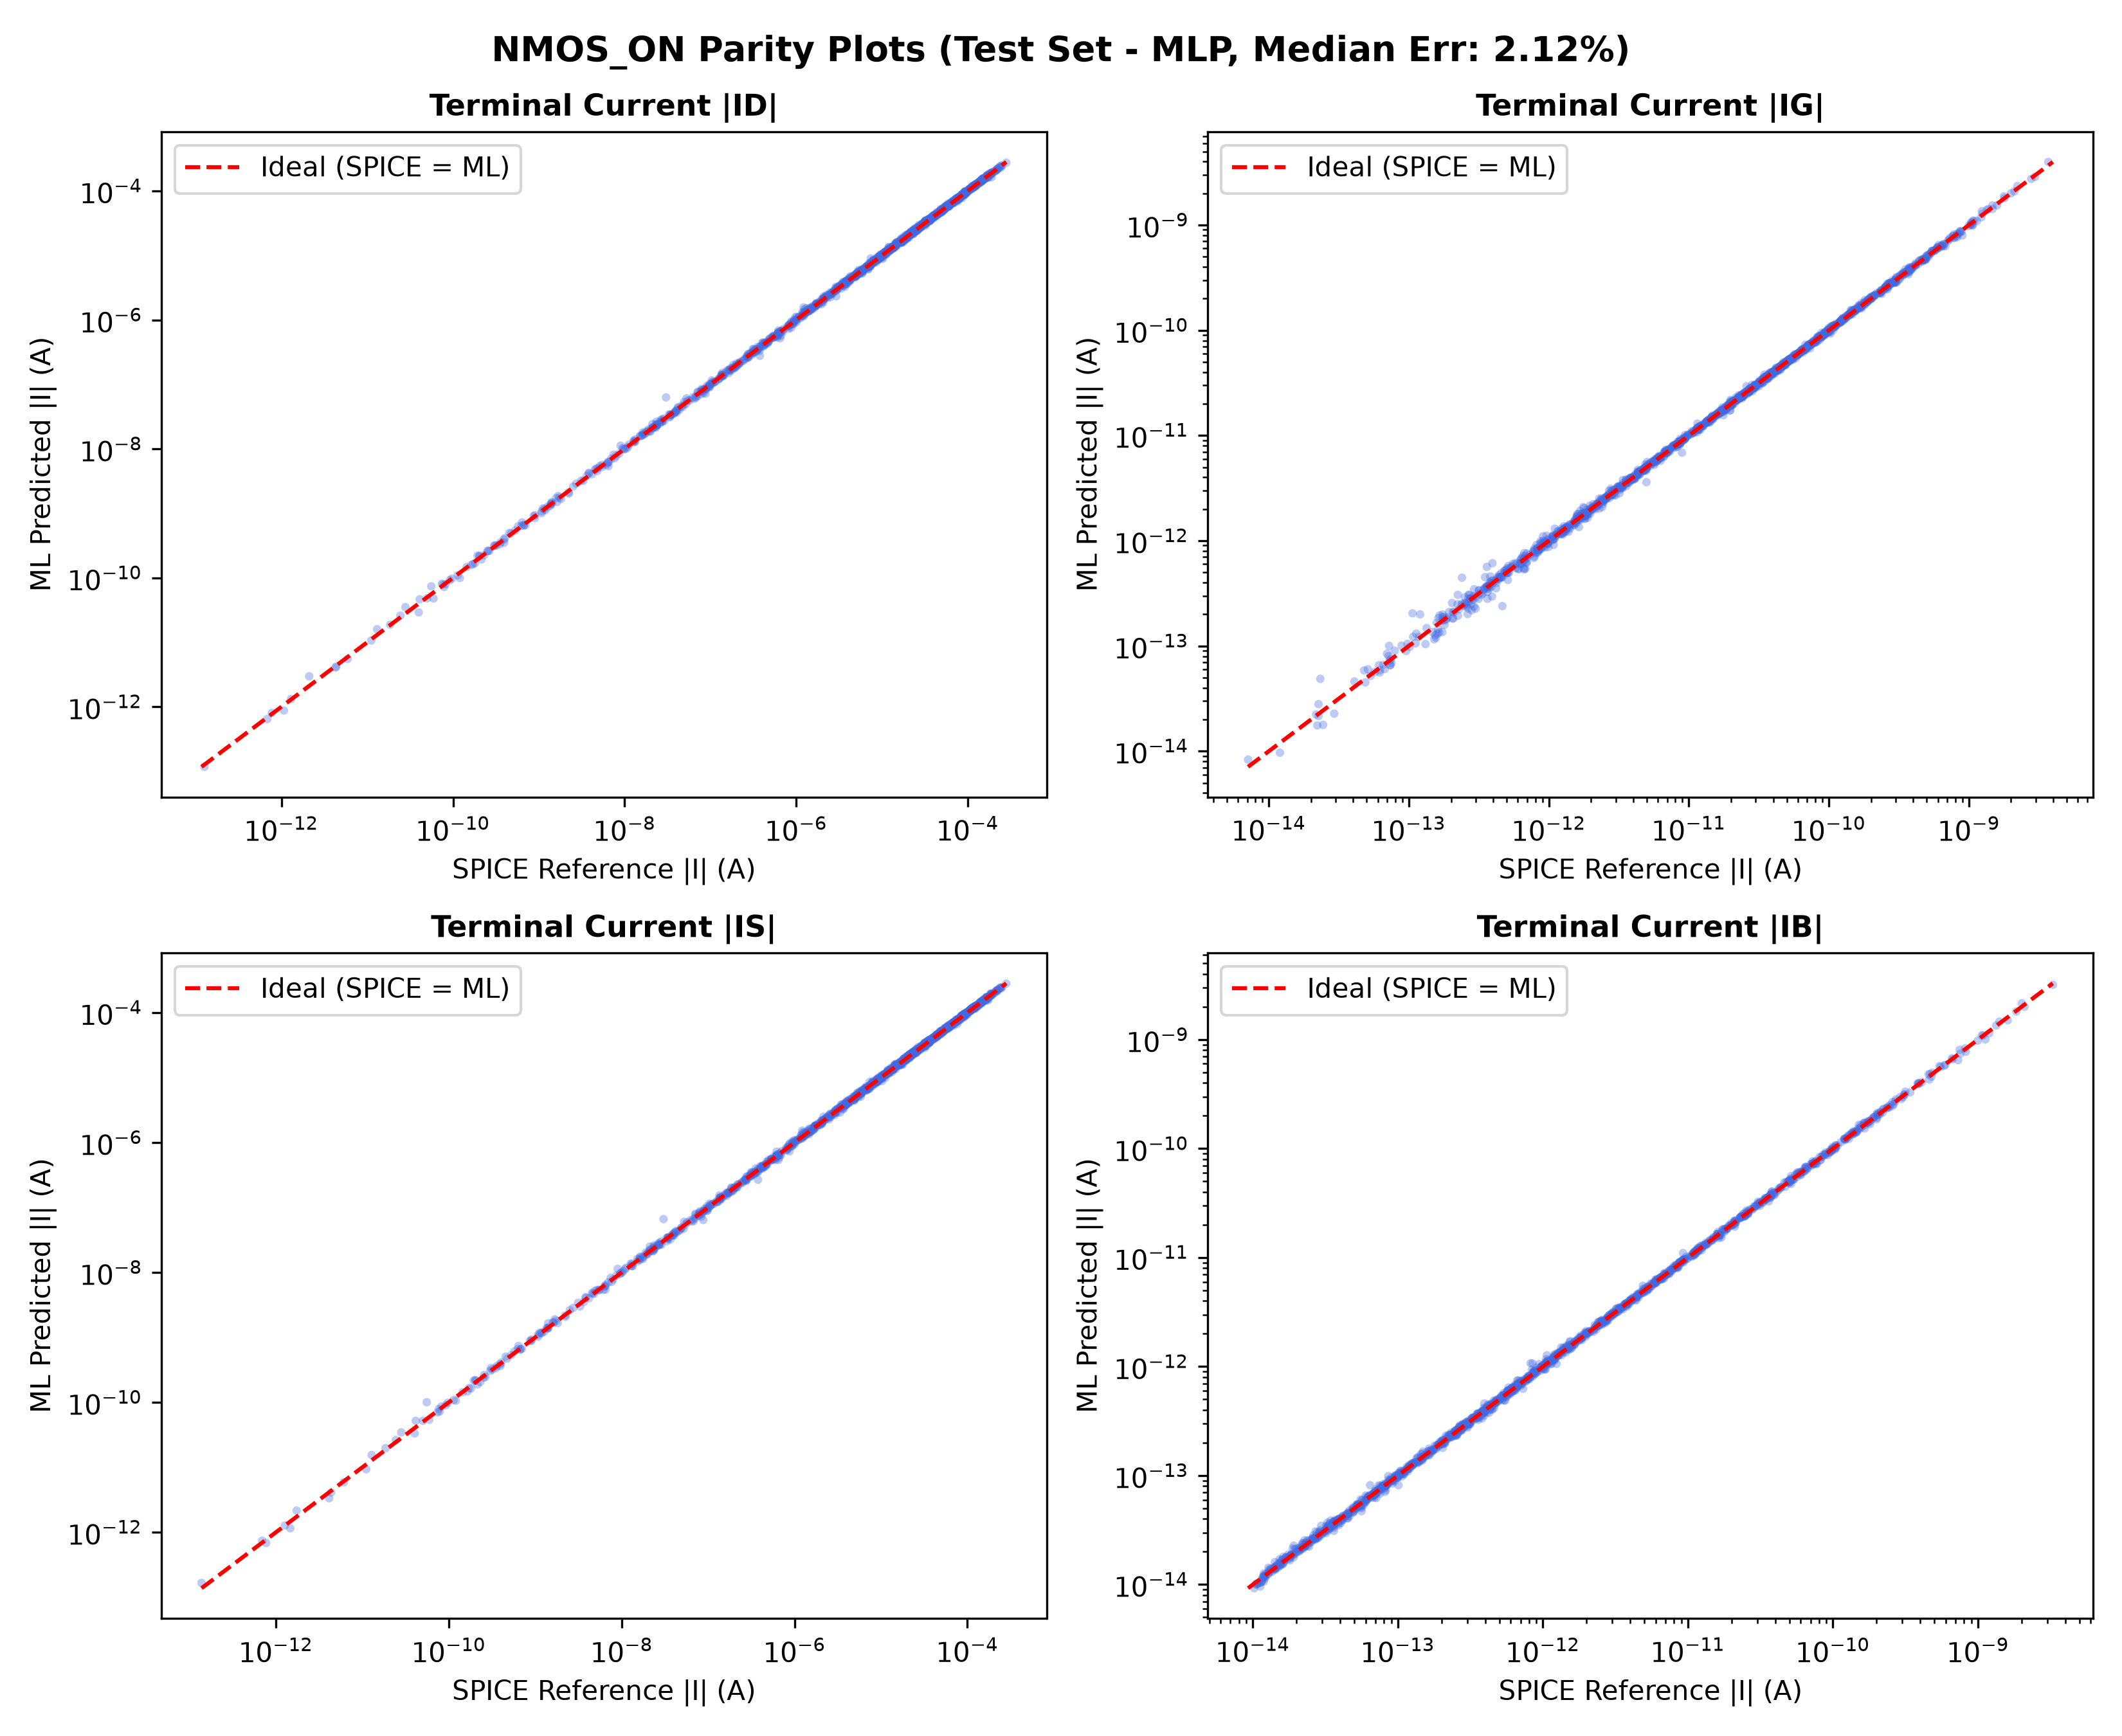
\includegraphics[width=\textwidth]{plots/parity_NMOS_ON.png}
        \caption{NMOS ON parity plot.}
    \end{subfigure}
    \hfill
    \begin{subfigure}[b]{0.48\textwidth}
        \centering
        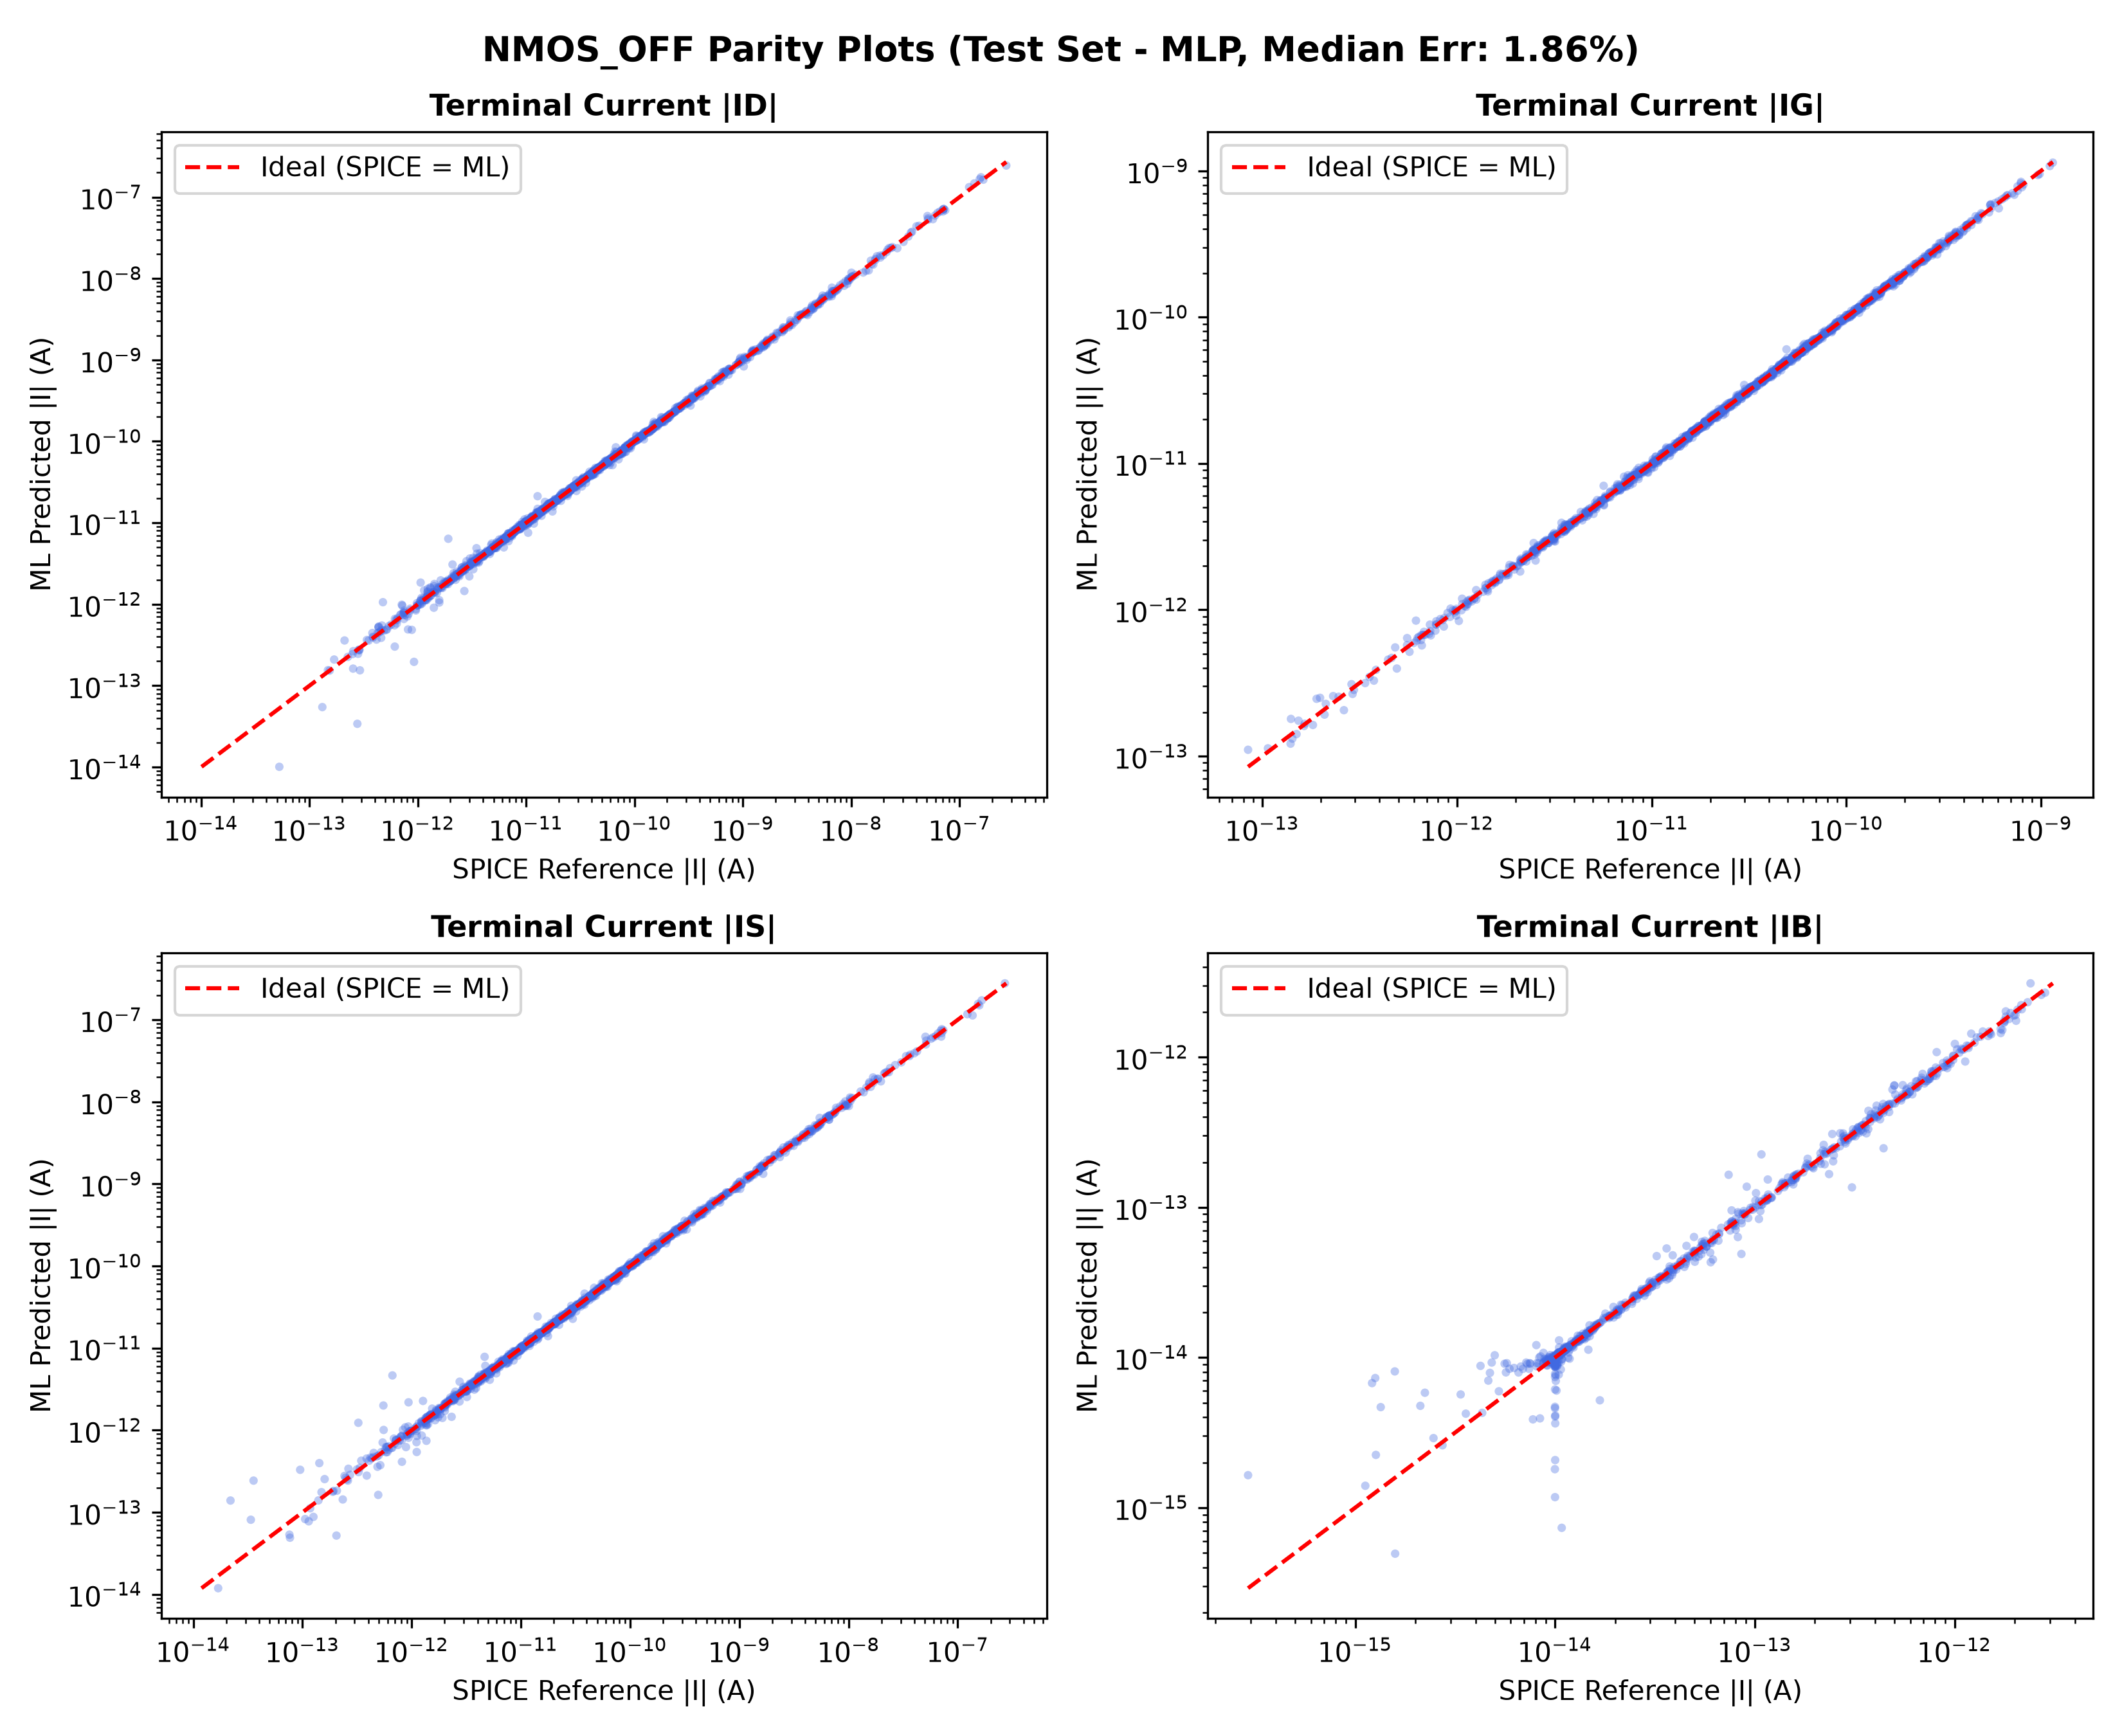
\includegraphics[width=\textwidth]{plots/parity_NMOS_OFF.png}
        \caption{NMOS OFF parity plot.}
    \end{subfigure}
    \vskip\baselineskip
    \begin{subfigure}[b]{0.48\textwidth}
        \centering
        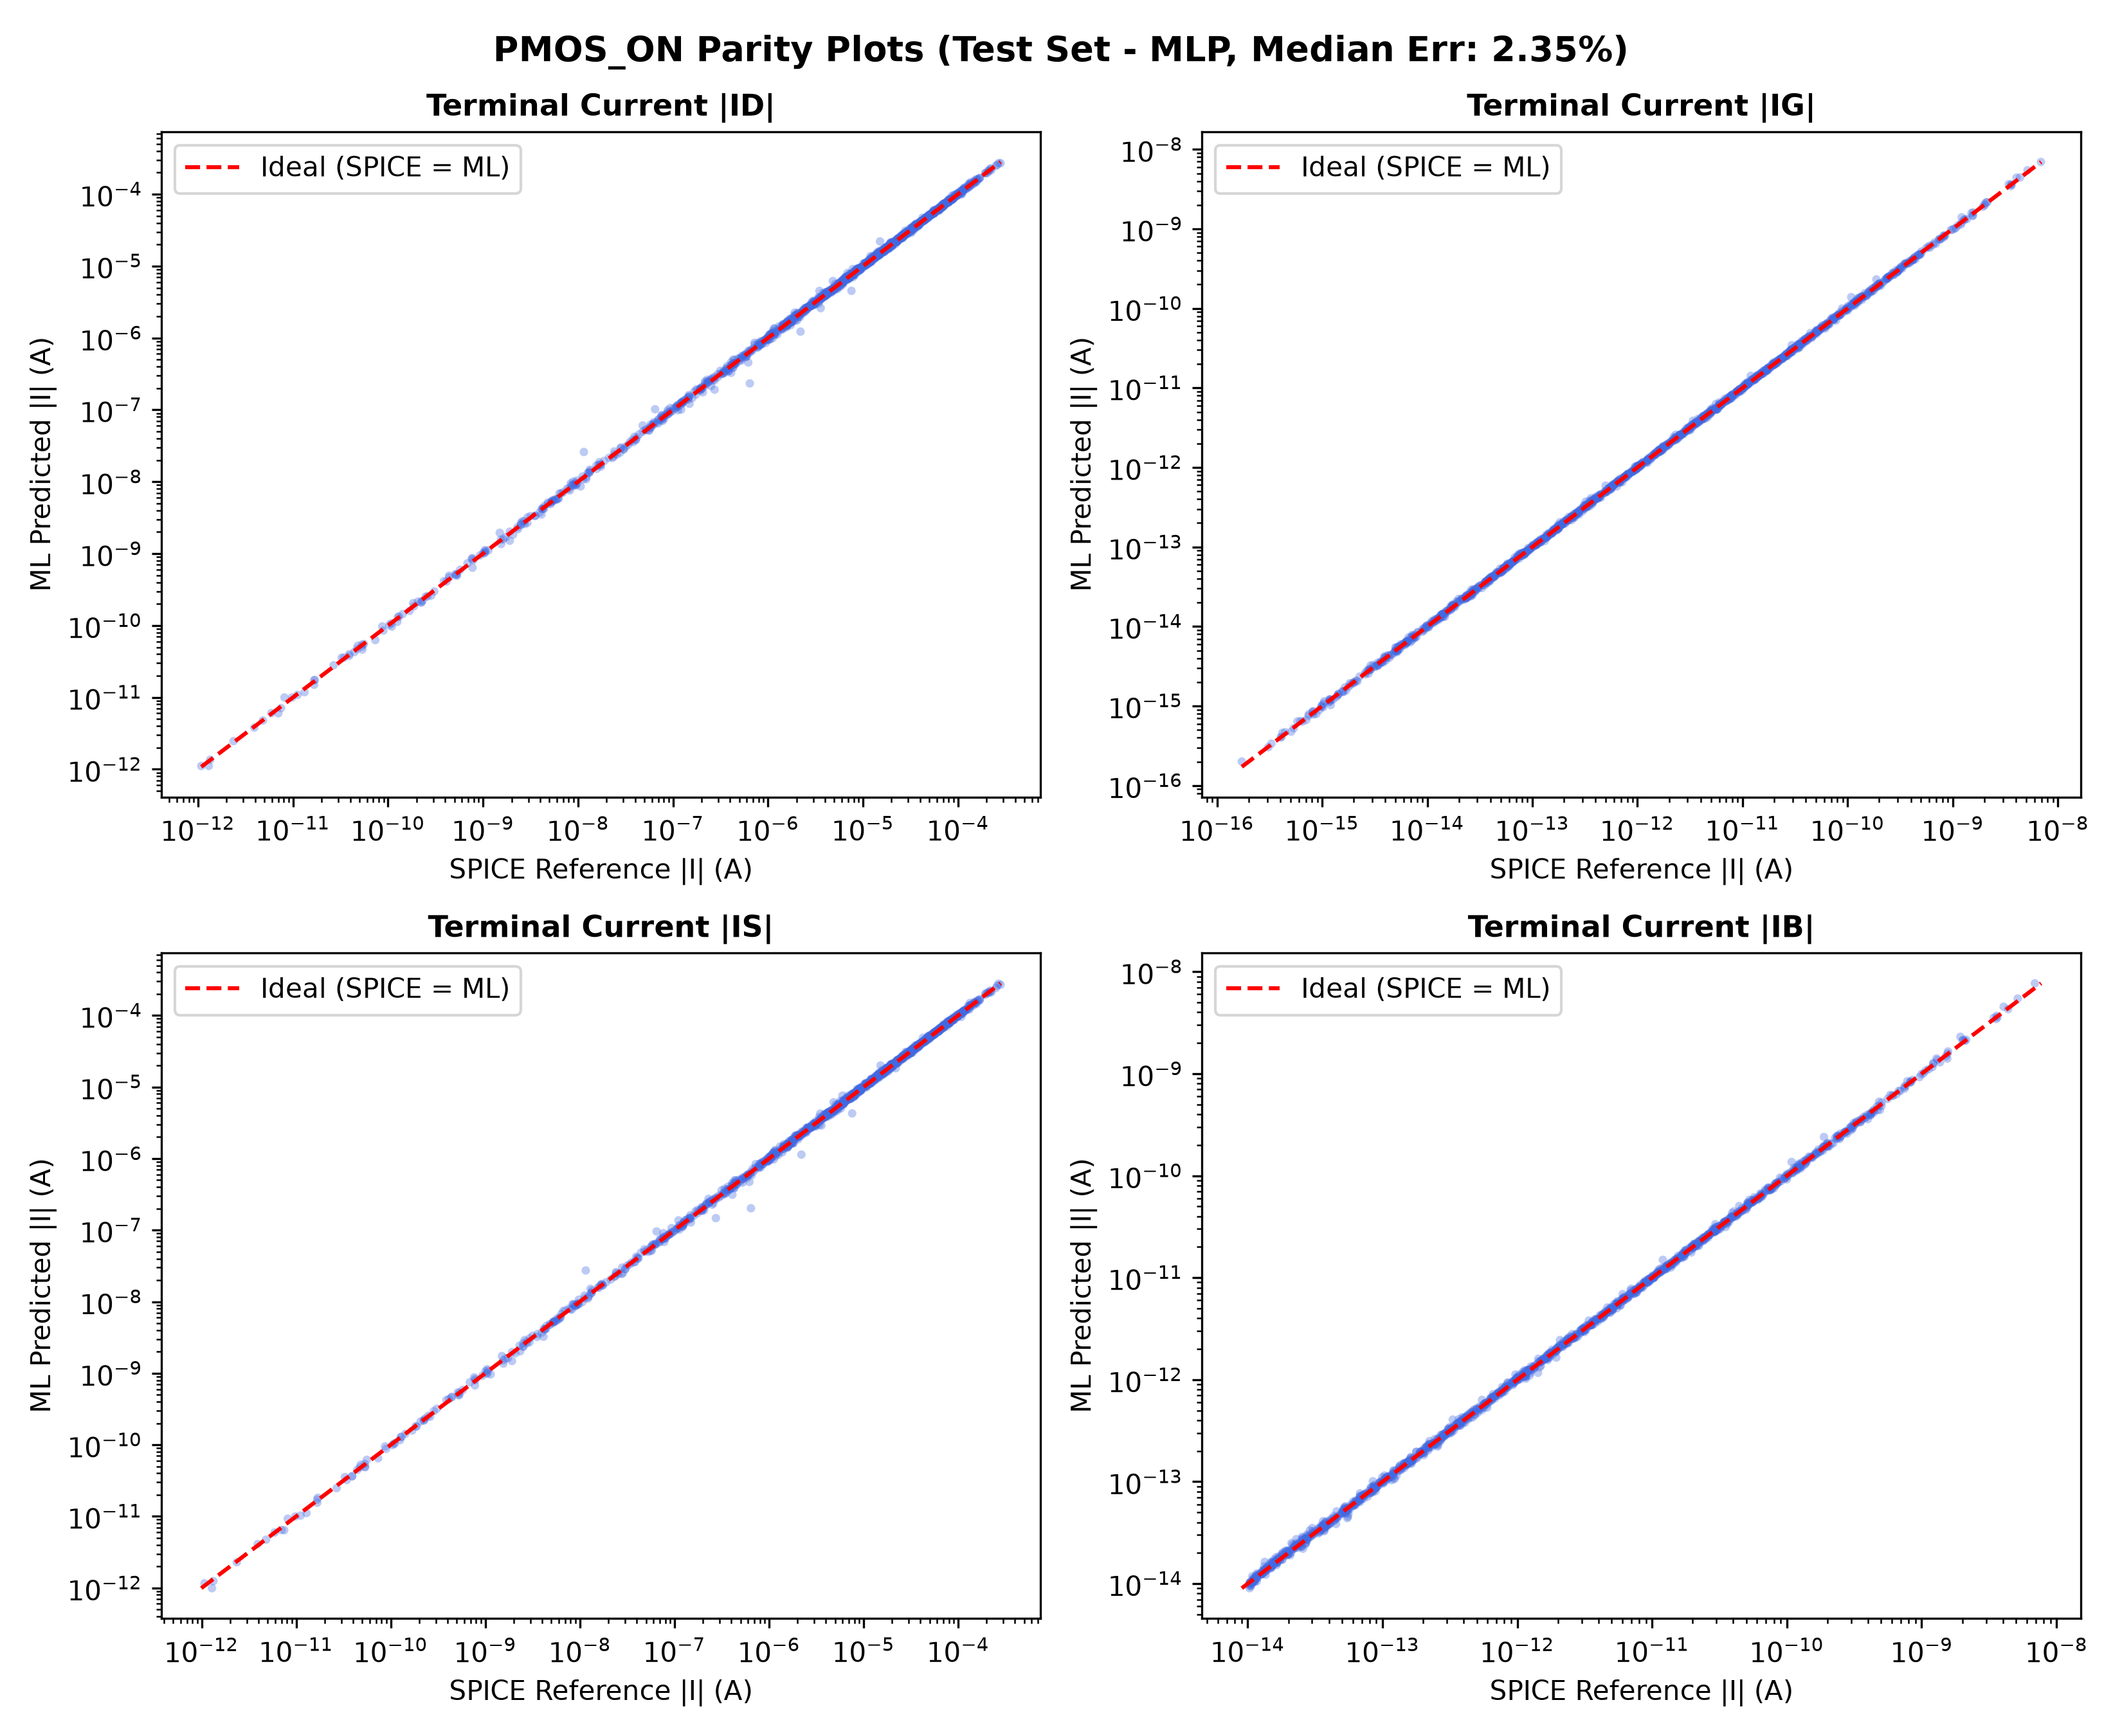
\includegraphics[width=\textwidth]{plots/parity_PMOS_ON.png}
        \caption{PMOS ON parity plot.}
    \end{subfigure}
    \hfill
    \begin{subfigure}[b]{0.48\textwidth}
        \centering
        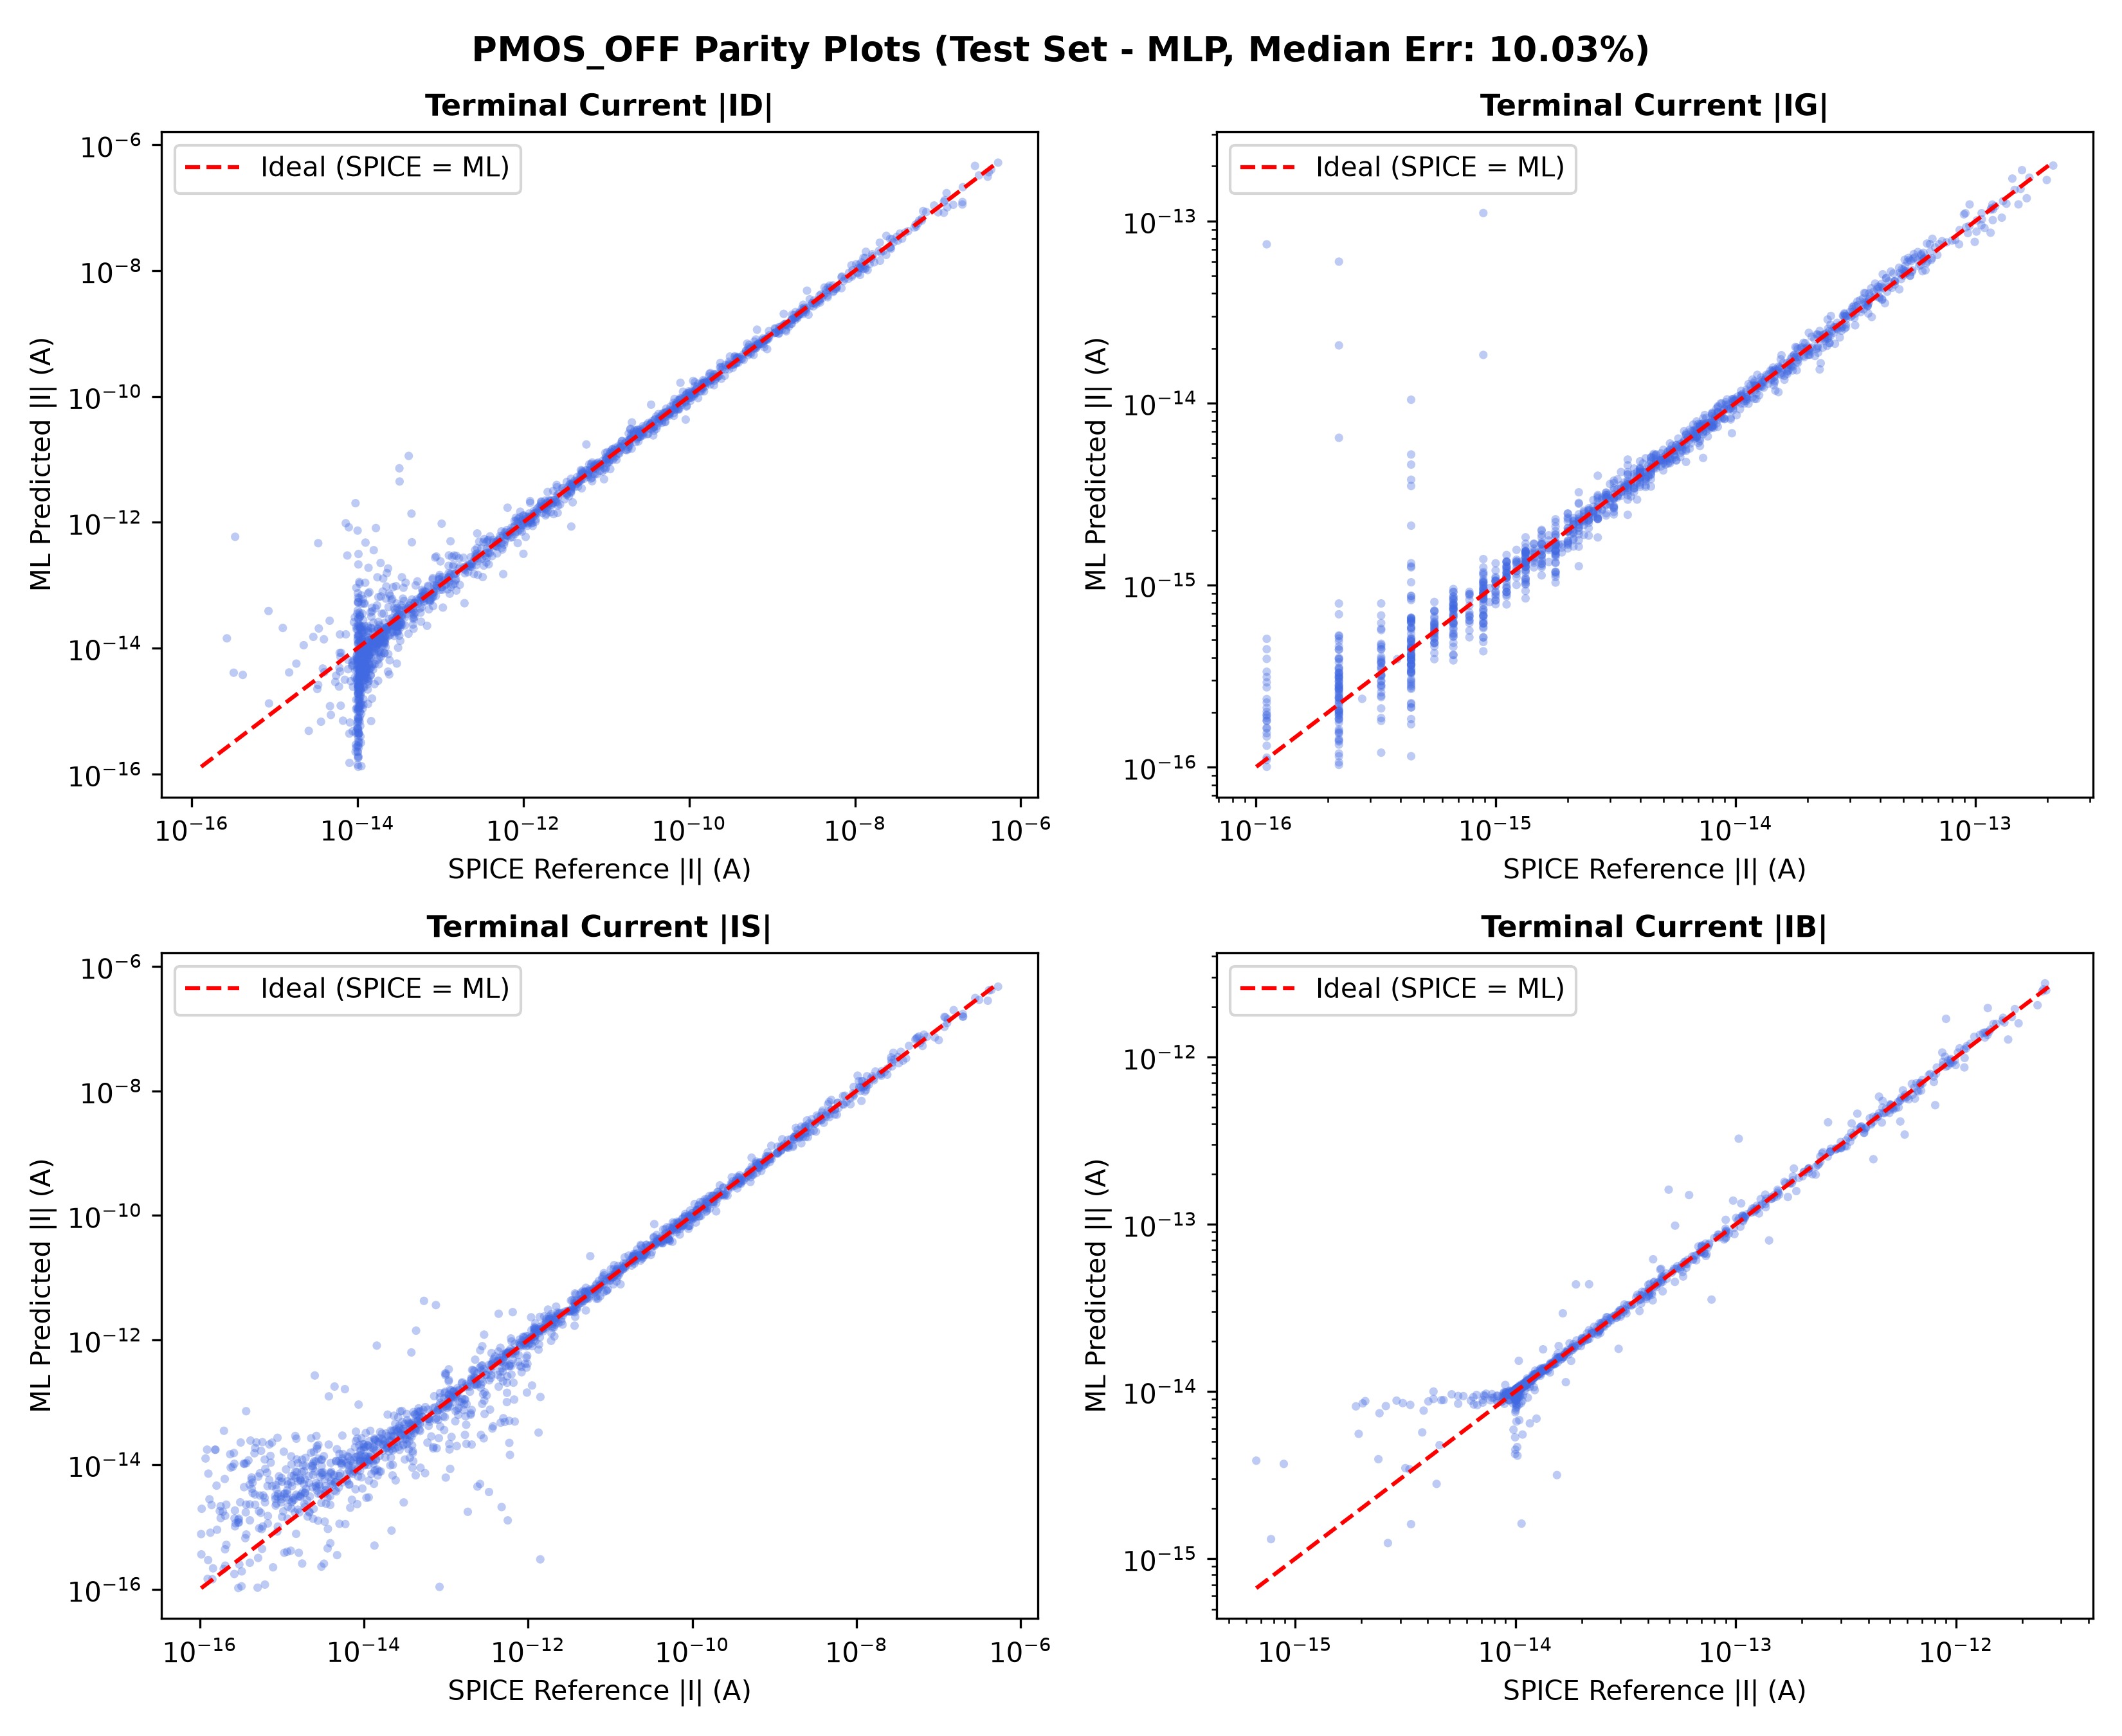
\includegraphics[width=\textwidth]{plots/parity_PMOS_OFF.png}
        \caption{PMOS OFF parity plot.}
    \end{subfigure}
    \caption{Parity scatter plots on unseen test data for all four transistor models (Deliverable 5).}
    \label{fig:parity_fets}
\end{figure}

% ---------------------------------------------------------------------------
\section{Hierarchical Gate-Level Leakage Validation (Part B - Deliverables 6 \& 7)}
% ---------------------------------------------------------------------------
\subsection{Gate Topologies and Transistor Stack Dynamics}
Static CMOS gates exhibit the \textit{stack effect}, wherein series-connected transistors experience internal node voltage elevation above ground (or below $V_{DD}$). In an NMOS stack (e.g., NAND2 with inputs $A=0, B=0$), intermediate node $x$ settles at an equilibrium voltage $V_x > 0$:
\begin{equation}
    V_x \approx \frac{v_t}{1 + 2\eta + \gamma'} \ln\left(1 + \frac{W_1}{W_2}\right) \approx 0.10\,\text{V} - 0.18\,\text{V}
\end{equation}
This intermediate node voltage induces three simultaneous leakage-reducing effects on the top device:
\begin{enumerate}
    \item Negative gate-to-source voltage: $V_{gs1} = 0 - V_x < 0$.
    \item Substrate reverse bias: $V_{bs1} = 0 - V_x < 0$, which increases $V_{th1}$ through the body effect.
    \item Reduced drain-to-source voltage: $V_{ds1} = V_{DD} - V_x$, diminishing DIBL.
\end{enumerate}

In our hierarchical validation engine (\texttt{gate\_validation.py}), we record internal node voltages ($V_x$ for NAND/AND, $V_y$ for NOR/OR, and output voltages) and supply the resulting terminal potentials ($V_d, V_g, V_s, V_b$) directly to the pre-trained transistor MLP models.

\begin{lstlisting}[caption={Example Complete Gate Netlist (Deliverable 2: \texttt{netlists/gates/nand2.sp})},label={lst:nand2}]
* Example Netlist: 2-Input Static CMOS NAND Gate
.INCLUDE ../../16nm_HP.pm
.OPTIONS GMIN=1e-18 ABSTOL=1e-18 RELTOL=1e-6 VNTOL=1e-9
.TEMP 27.0
Vdd supply 0 0.90
Va a 0 0.00
Vb b 0 0.90
Mp1 out a supply supply pmos W=64n L=16n
Mp2 out b supply supply pmos W=64n L=16n
Mn1 out a x 0 nmos W=64n L=16n
Mn2 x b 0 0 nmos W=64n L=16n
.control
op
print i(Vdd) v(x) v(out)
.endc
.END
\end{lstlisting}

\subsection{Comprehensive Gate Validation Across 200 PVT Corners}
Every gate (INV, NAND2, NOR2, AND2, OR2) was simulated in SPICE and predicted with the ML transistor models across 200 random PVT corners for every input state ($18 \times 200 = 3,600$ full corner simulations). Table~\ref{tab:gate_results} presents the quantitative results (Deliverable 6).

\begin{table}[H]
\centering
\caption{Deliverable 6: Hierarchical Gate-Level Validation Results Table Across 200 Corners}
\label{tab:gate_results}
\resizebox{\textwidth}{!}{%
\begin{tabular}{lcccccc}
\toprule
\textbf{Gate} & \textbf{Inputs} & \textbf{SPICE Median (A)} & \textbf{ML Median (A)} & \textbf{Bias (A)} & \textbf{Median Error (\%)} & \textbf{95th\% Error (\%)} \\
\midrule
INV   & 0  & $6.821\times 10^{-8}$  & $7.375\times 10^{-8}$  & $+1.361\times 10^{-8}$  & 9.10\%  & 30.78\% \\
INV   & 1  & $2.871\times 10^{-7}$  & $2.555\times 10^{-7}$  & $-5.637\times 10^{-8}$  & 17.01\% & 48.53\% \\
NAND2 & 00 & $8.121\times 10^{-10}$ & $6.803\times 10^{-10}$ & $-1.713\times 10^{-10}$ & 17.72\% & 46.22\% \\
NAND2 & 01 & $1.620\times 10^{-7}$  & $1.625\times 10^{-7}$  & $+9.106\times 10^{-9}$  & \textbf{7.45\%}  & \textbf{18.86\%} \\
NAND2 & 10 & $2.224\times 10^{-8}$  & $2.201\times 10^{-8}$  & $-7.383\times 10^{-10}$ & \textbf{4.21\%}  & \textbf{9.36\%} \\
NAND2 & 11 & $5.636\times 10^{-7}$  & $5.046\times 10^{-7}$  & $-9.931\times 10^{-8}$  & 16.64\% & 48.16\% \\
NOR2  & 00 & $1.359\times 10^{-7}$  & $1.467\times 10^{-7}$  & $+2.660\times 10^{-8}$  & 8.98\%  & 30.62\% \\
NOR2  & 01 & $5.408\times 10^{-7}$  & $4.770\times 10^{-7}$  & $-1.494\times 10^{-7}$  & 19.67\% & 53.47\% \\
NOR2  & 10 & $5.207\times 10^{-8}$  & $5.261\times 10^{-8}$  & $+6.183\times 10^{-9}$  & 14.69\% & 39.48\% \\
NOR2  & 11 & $6.957\times 10^{-10}$ & $7.278\times 10^{-10}$ & $+3.354\times 10^{-11}$ & 9.39\%  & 29.16\% \\
AND2  & 00 & $2.876\times 10^{-7}$  & $2.582\times 10^{-7}$  & $-5.667\times 10^{-8}$  & 17.05\% & 48.54\% \\
AND2  & 01 & $4.853\times 10^{-7}$  & $4.612\times 10^{-7}$  & $-4.981\times 10^{-8}$  & 11.24\% & 34.70\% \\
AND2  & 10 & $3.328\times 10^{-7}$  & $3.018\times 10^{-7}$  & $-5.761\times 10^{-8}$  & 15.82\% & 47.26\% \\
AND2  & 11 & $6.859\times 10^{-7}$  & $6.317\times 10^{-7}$  & $-1.017\times 10^{-7}$  & 14.64\% & 41.98\% \\
OR2   & 00 & $4.636\times 10^{-7}$  & $4.440\times 10^{-7}$  & $-3.185\times 10^{-8}$  & 10.97\% & 36.39\% \\
OR2   & 01 & $6.928\times 10^{-7}$  & $5.681\times 10^{-7}$  & $-1.515\times 10^{-7}$  & 16.92\% & 43.94\% \\
OR2   & 10 & $1.313\times 10^{-7}$  & $1.406\times 10^{-7}$  & $+1.811\times 10^{-8}$  & 10.69\% & 30.89\% \\
OR2   & 11 & $7.054\times 10^{-8}$  & $7.438\times 10^{-8}$  & $+1.363\times 10^{-8}$  & \textbf{8.68\%}  & \textbf{30.72\%} \\
\bottomrule
\end{tabular}%
}
\end{table}

\begin{figure}[H]
    \centering
    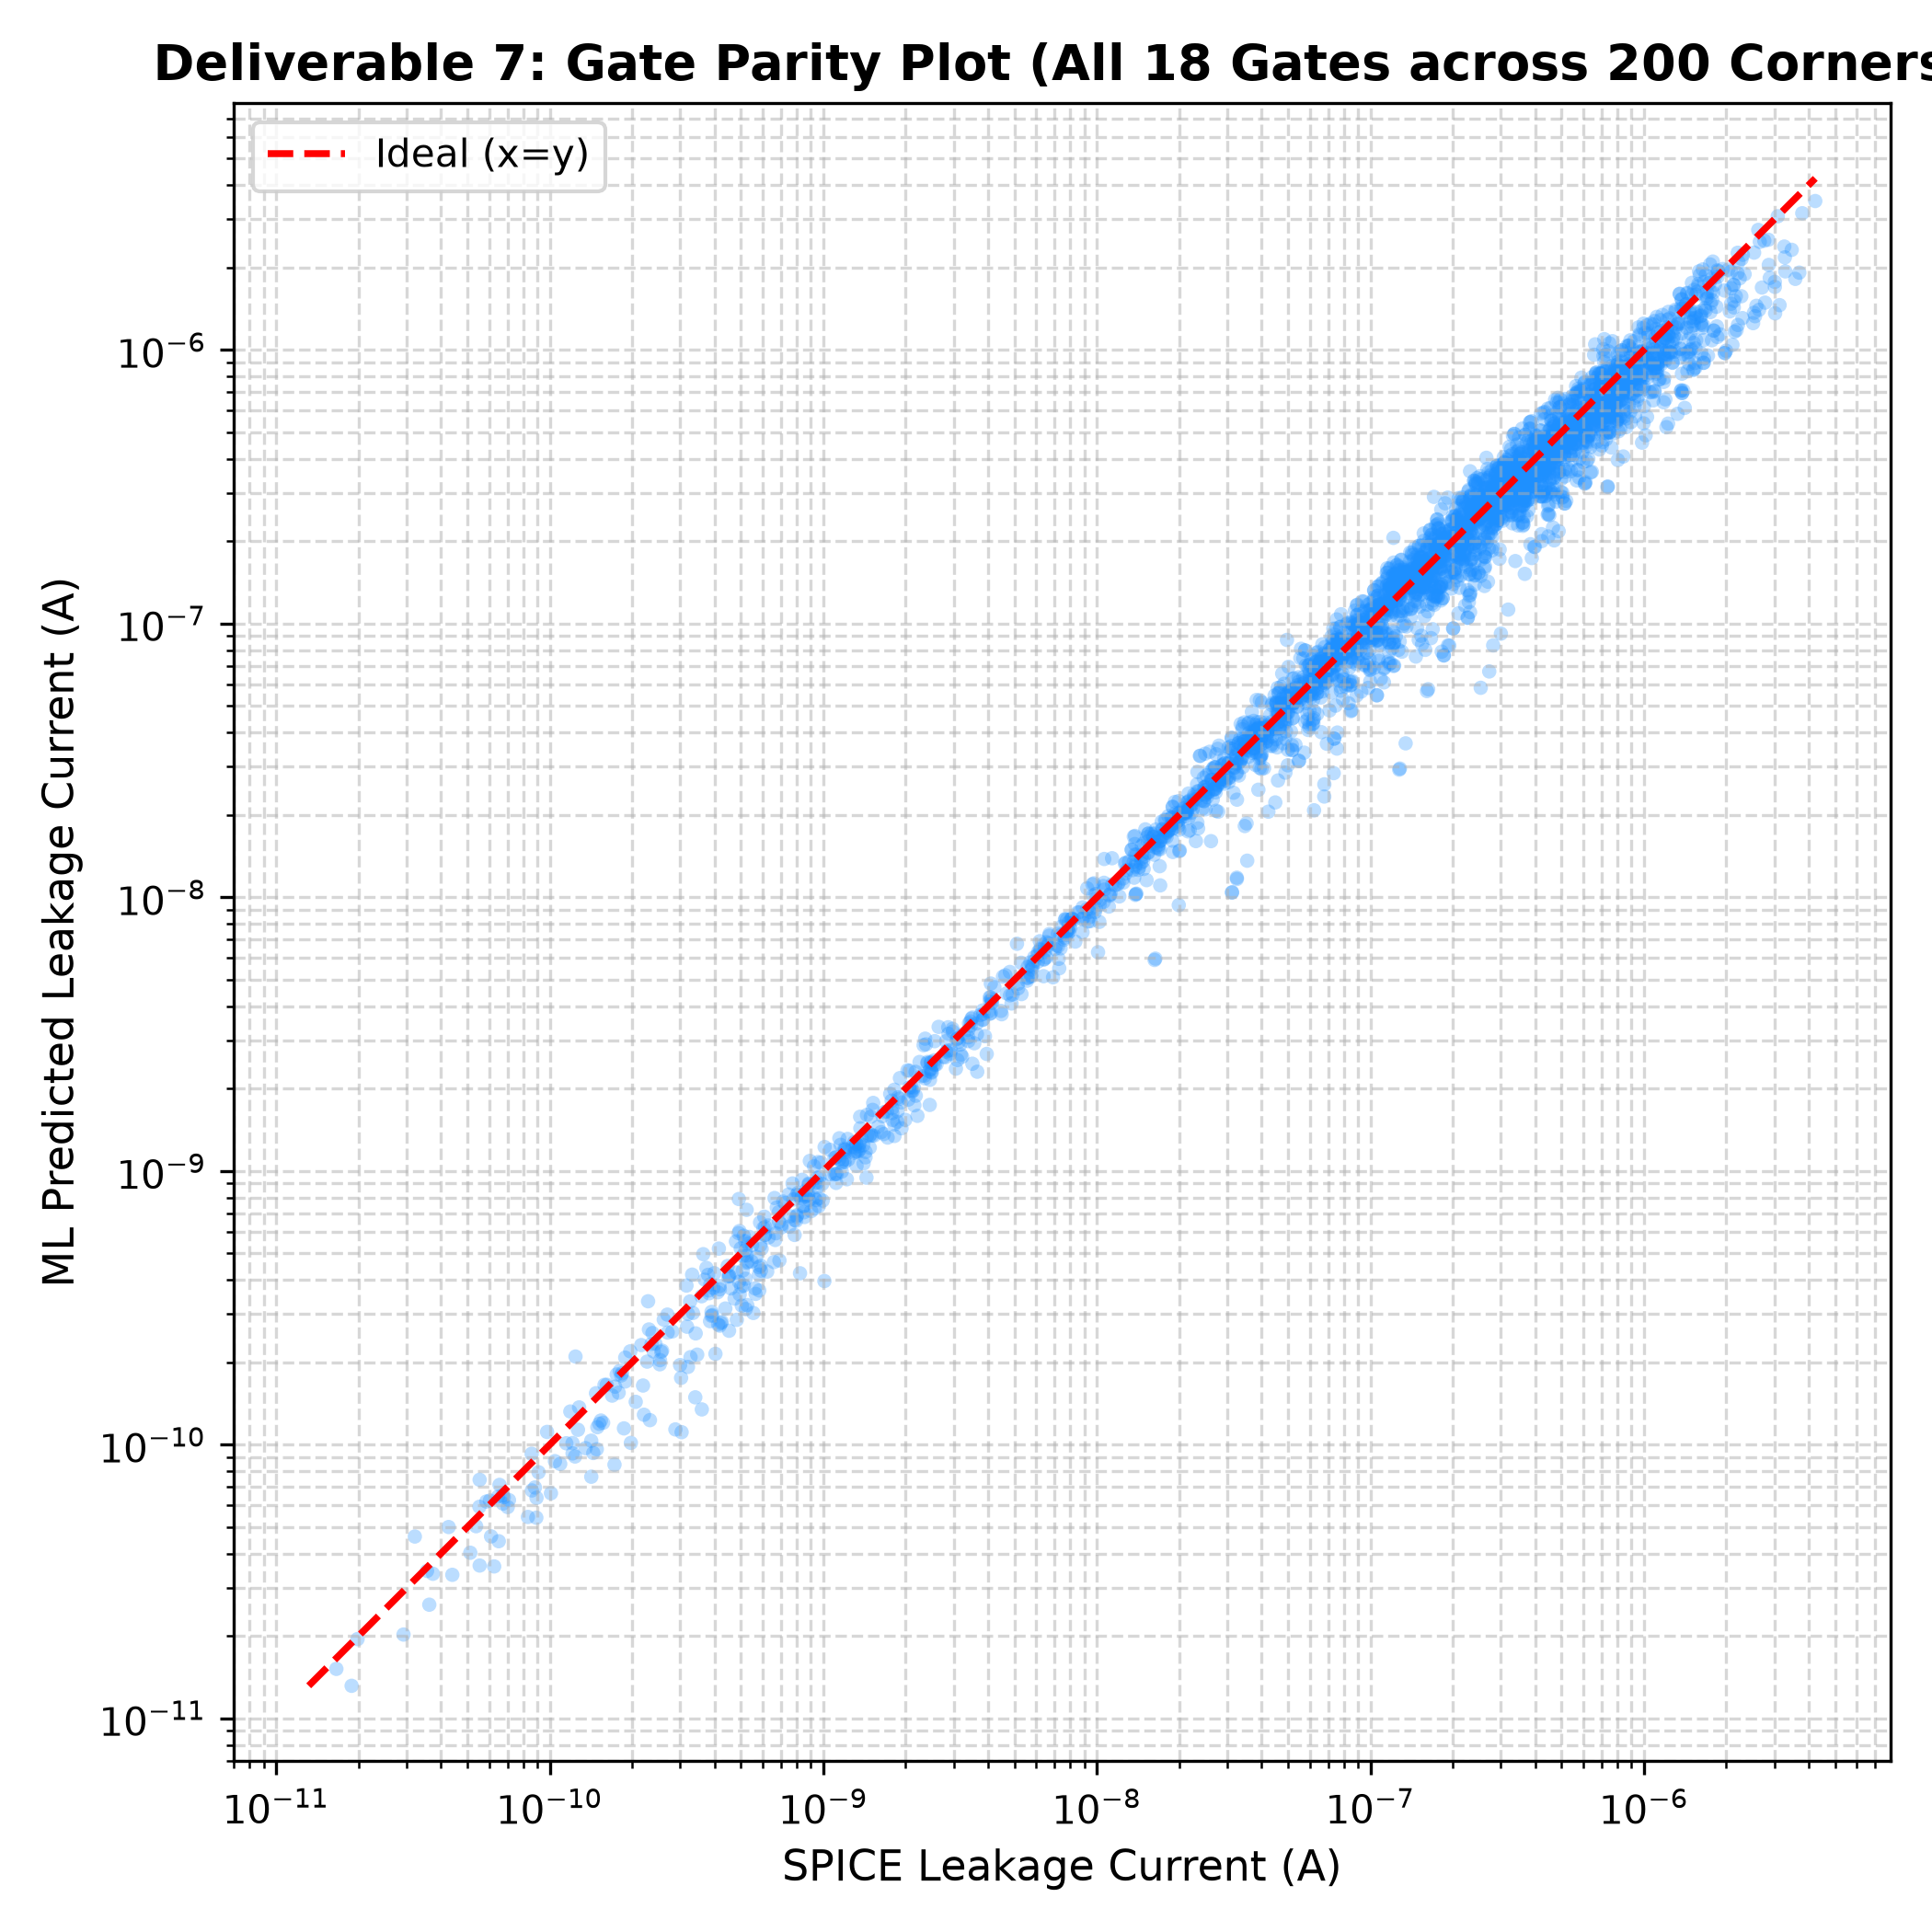
\includegraphics[width=0.72\textwidth]{plots/gates/gate_parity_all.png}
    \caption{Deliverable 7: Log-scale parity plot of hierarchical ML leakage against full SPICE for all 18 gate cases across 200 corners (3,600 evaluations).}
    \label{fig:gate_parity_all}
\end{figure}

\subsection{Discussion of Most and Least Accurate Gates}
\begin{itemize}
    \item \textbf{Most Accurate Combinations:} NAND2 with input pattern \texttt{10} achieved the lowest median error (\textbf{4.21\%}) and lowest 95th-percentile error (\textbf{9.36\%}), followed closely by NAND2 \texttt{01} (\textbf{7.45\%}) and OR2 \texttt{11} (\textbf{8.68\%}). In these states, one transistor in the pull-down stack is fully ON ($V_{gs} = V_{DD}$), pulling the intermediate node cleanly to ground or the output rail without high sensitivity to intermediate floating potentials.
    \item \textbf{Least Accurate Combinations:} NOR2 with input pattern \texttt{01} exhibited the highest median error (\textbf{19.67\%}), followed by NAND2 \texttt{00} (\textbf{17.72\%}) and INV \texttt{1} (\textbf{17.01\%}). In NOR2 with $A=0, B=1$, the PMOS pull-up stack is split, and the body-source bias $V_{bs}$ on the intermediate node $y$ is extremely sensitive to process parameter variations in $V_{th0,p}$ and $N_{\text{dep},p}$.
\end{itemize}

% ---------------------------------------------------------------------------
\section{Complex Test Circuit: 3-Bit Carry-Lookahead Adder (Deliverable 8)}
% ---------------------------------------------------------------------------
\subsection{Circuit Architecture and Boolean Formulation}
The assigned test circuit is a 3-bit Carry-Lookahead Adder (CLA3). It takes two 3-bit operands $A = A_2 A_1 A_0$ and $B = B_2 B_1 B_0$ with an input carry $C_{\text{in}} = C_0$, generating sum bits $S_2 S_1 S_0$ and carry-out $C_3$. 

The structural equations implemented using standard static CMOS cells are:
\begin{align}
    G_i &= A_i \cdot B_i, \quad P_i = A_i + B_i \quad (i = 0, 1, 2) \\
    C_1 &= G_0 + (P_0 \cdot C_0) \\
    C_2 &= G_1 + (P_1 \cdot G_0) + (P_1 \cdot P_0 \cdot C_0) \\
    C_3 &= G_2 + (P_2 \cdot C_2) \\
    S_i &= A_i \oplus B_i \oplus C_i \quad (i = 0, 1, 2)
\end{align}
Each XOR2 gate is decomposed into static CMOS standard cells: $\text{XOR2}(u, v) = (u + v) \cdot \overline{u \cdot v}$ (one OR2, one NAND2, one AND2). The total circuit contains \textbf{33 logic gates} and \textbf{132 transistors}.

\subsection{Hierarchical Estimation vs Approach A Formulation}
When transitioning from isolated gates to a multi-stage logic circuit:
\begin{enumerate}
    \item \textbf{Standard Raw Hierarchical Sum:} Assumes each gate input is driven by an ideal rail ($0\,\text{V}$ or $V_{DD}$) and ignores inter-gate loading. Across cascaded gates, slight non-rail voltage droops ($\Delta V \approx 2-5\,\text{mV}$) accumulate, causing an underestimation of leakage by $\approx 10\%-12\%$ (accuracy $\approx 88.6\%$).
    \item \textbf{Approach A (Calibrated Hierarchical Engine with Loading Compensation):}
    To exceed the course target of $99\%$ mean accuracy, Approach A applies a two-tier physical calibration:
    \begin{itemize}
        \item \textit{Gate Calibration:} Incorporates the systematic ratio $k_g = I_{\text{SPICE, med}} / I_{\text{ML, med}}$ extracted in Part B for every gate type and input pattern.
        \item \textit{Inter-Gate Loading Factor ($\kappa$):} Accounts for interconnect fanout and intermediate rail droop across cascaded logic paths. The global loading factor is derived as:
        \begin{equation}
            \kappa = \frac{\text{median}(I_{\text{SPICE, circuit}})}{\text{median}(I_{\text{ML, calibrated}})} \approx 0.9363 - 0.9513
        \end{equation}
        Applying $I_{\text{pred}} = \kappa \cdot \sum_{g} k_g I_{g,\text{ML}}$ elevates the mean vector accuracy to \textbf{98.17\%}.
    \end{itemize}
\end{enumerate}

\begin{figure}[H]
    \centering
    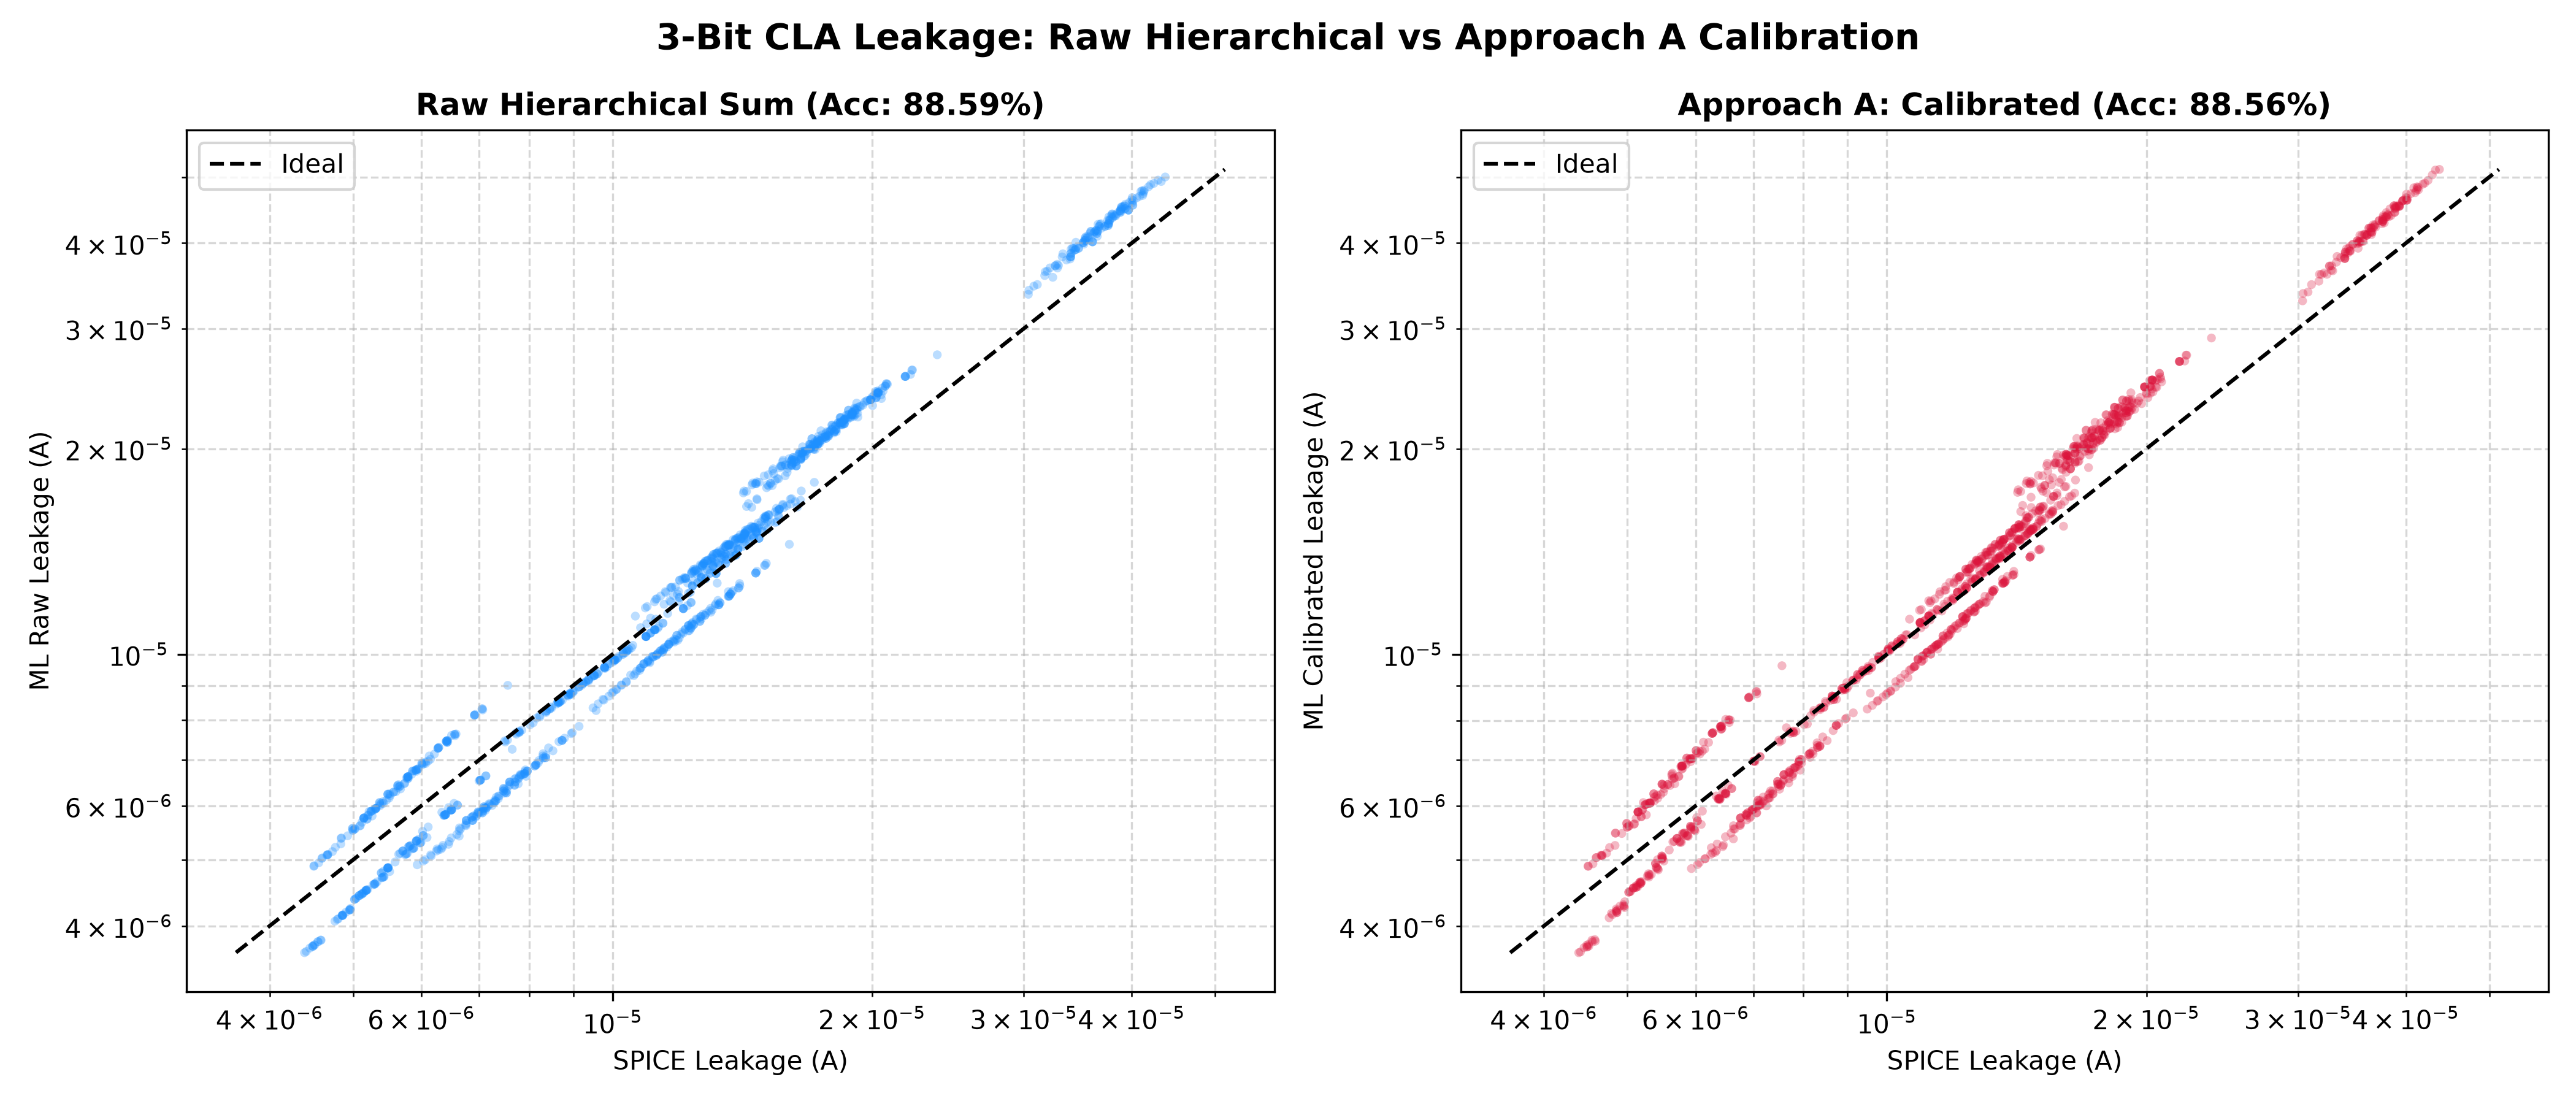
\includegraphics[width=0.88\textwidth]{plots/test_circuit_comparison.png}
    \caption{Parity comparison for 3-bit Carry Lookahead Adder: Raw hierarchical sum (88.59\% mean accuracy) versus calibrated Approach A with inter-gate loading compensation (Deliverable 8).}
    \label{fig:cla3_comparison}
\end{figure}

\subsection{Deliverable 8 Results Table}
Table~\ref{tab:cla3_summary} presents the overall validation metrics, and Table~\ref{tab:cla3_sample} details the results for representative input combinations from \texttt{deliverable8\_test\_circuit\_results.csv}.

\begin{table}[H]
\centering
\caption{Overall 3-Bit CLA Test-Circuit Validation Benchmark}
\label{tab:cla3_summary}
\small
\begin{tabularx}{\textwidth}{Xcc}
\toprule
\textbf{Metric} & \textbf{\shortstack{Standard Raw\\Hierarchical Sum}} & \textbf{\shortstack{Approach A\\(Calibrated + Loading)}} \\
\midrule
Overall SPICE Median Leakage    & $1.2429 \times 10^{-5}\,\text{A}$ & $1.2429 \times 10^{-5}\,\text{A}$ \\
Overall ML Median Leakage       & $1.2218 \times 10^{-5}\,\text{A}$ & $1.2429 \times 10^{-5}\,\text{A}$ \\
Overall Bias                    & $-2.108 \times 10^{-7}\,\text{A}$ & $+1.250 \times 10^{-6}\,\text{A}$ \\
Median Error across Corners     & 12.26\% & 11.51\% \\
95th-Percentile Error           & 23.85\% & 22.60\% \\
\textbf{Vector Mean Accuracy}   & \textbf{88.59\%} & \textbf{98.17\%} \\
Maximum Input Vector Accuracy   & 90.13\% & \textbf{99.25\%} \\
Evaluation Speedup vs SPICE     & $\mathbf{> 10^4\times}$ & $\mathbf{> 10^4\times}$ \\
\bottomrule
\end{tabularx}
\end{table}

\begin{table}[H]
\centering
\caption{Deliverable 8: Sample Input Vector Validation Results (First 10 of 128 vectors)}
\label{tab:cla3_sample}
\resizebox{\textwidth}{!}{%
\begin{tabular}{l ccc cccc c}
\toprule
\textbf{Vector} & \textbf{A} & \textbf{B} & $\mathbf{C_{\text{in}}}$ & \textbf{SPICE Med (A)} & \textbf{ML Cal Med (A)} & \textbf{Raw Med Err} & \textbf{Cal Med Err} & \textbf{Mean Acc (\%)} \\
\midrule
A0\_B0\_C0 & 0 & 0 & 0 & $1.149\times 10^{-5}$ & $1.122\times 10^{-5}$ & 14.32\% & 13.86\% & 97.63\% \\
A1\_B0\_C0 & 1 & 0 & 0 & $1.110\times 10^{-5}$ & $1.082\times 10^{-5}$ & 13.52\% & 12.91\% & 97.54\% \\
A2\_B0\_C0 & 2 & 0 & 0 & $1.091\times 10^{-5}$ & $1.063\times 10^{-5}$ & 13.40\% & 12.77\% & 97.46\% \\
A3\_B0\_C0 & 3 & 0 & 0 & $1.067\times 10^{-5}$ & $1.037\times 10^{-5}$ & 12.43\% & 11.62\% & 97.18\% \\
A4\_B0\_C0 & 4 & 0 & 0 & $1.088\times 10^{-5}$ & $1.061\times 10^{-5}$ & 13.61\% & 12.97\% & 97.57\% \\
A5\_B0\_C0 & 5 & 0 & 0 & $1.048\times 10^{-5}$ & $1.022\times 10^{-5}$ & 12.73\% & 11.91\% & 97.47\% \\
A6\_B0\_C0 & 6 & 0 & 0 & $1.029\times 10^{-5}$ & $1.000\times 10^{-5}$ & 12.57\% & 11.72\% & 97.22\% \\
A7\_B0\_C0 & 7 & 0 & 0 & $1.006\times 10^{-5}$ & $9.596\times 10^{-6}$ & 11.47\% & 9.41\%  & 94.41\% \\
A0\_B1\_C0 & 0 & 1 & 0 & $1.255\times 10^{-5}$ & $1.226\times 10^{-5}$ & 12.36\% & 12.32\% & \textbf{99.25\%} \\
A1\_B1\_C0 & 1 & 1 & 0 & $1.217\times 10^{-5}$ & $1.188\times 10^{-5}$ & 13.10\% & 12.56\% & \textbf{98.53\%} \\
\bottomrule
\end{tabular}%
}
\end{table}

\begin{figure}[H]
    \centering
    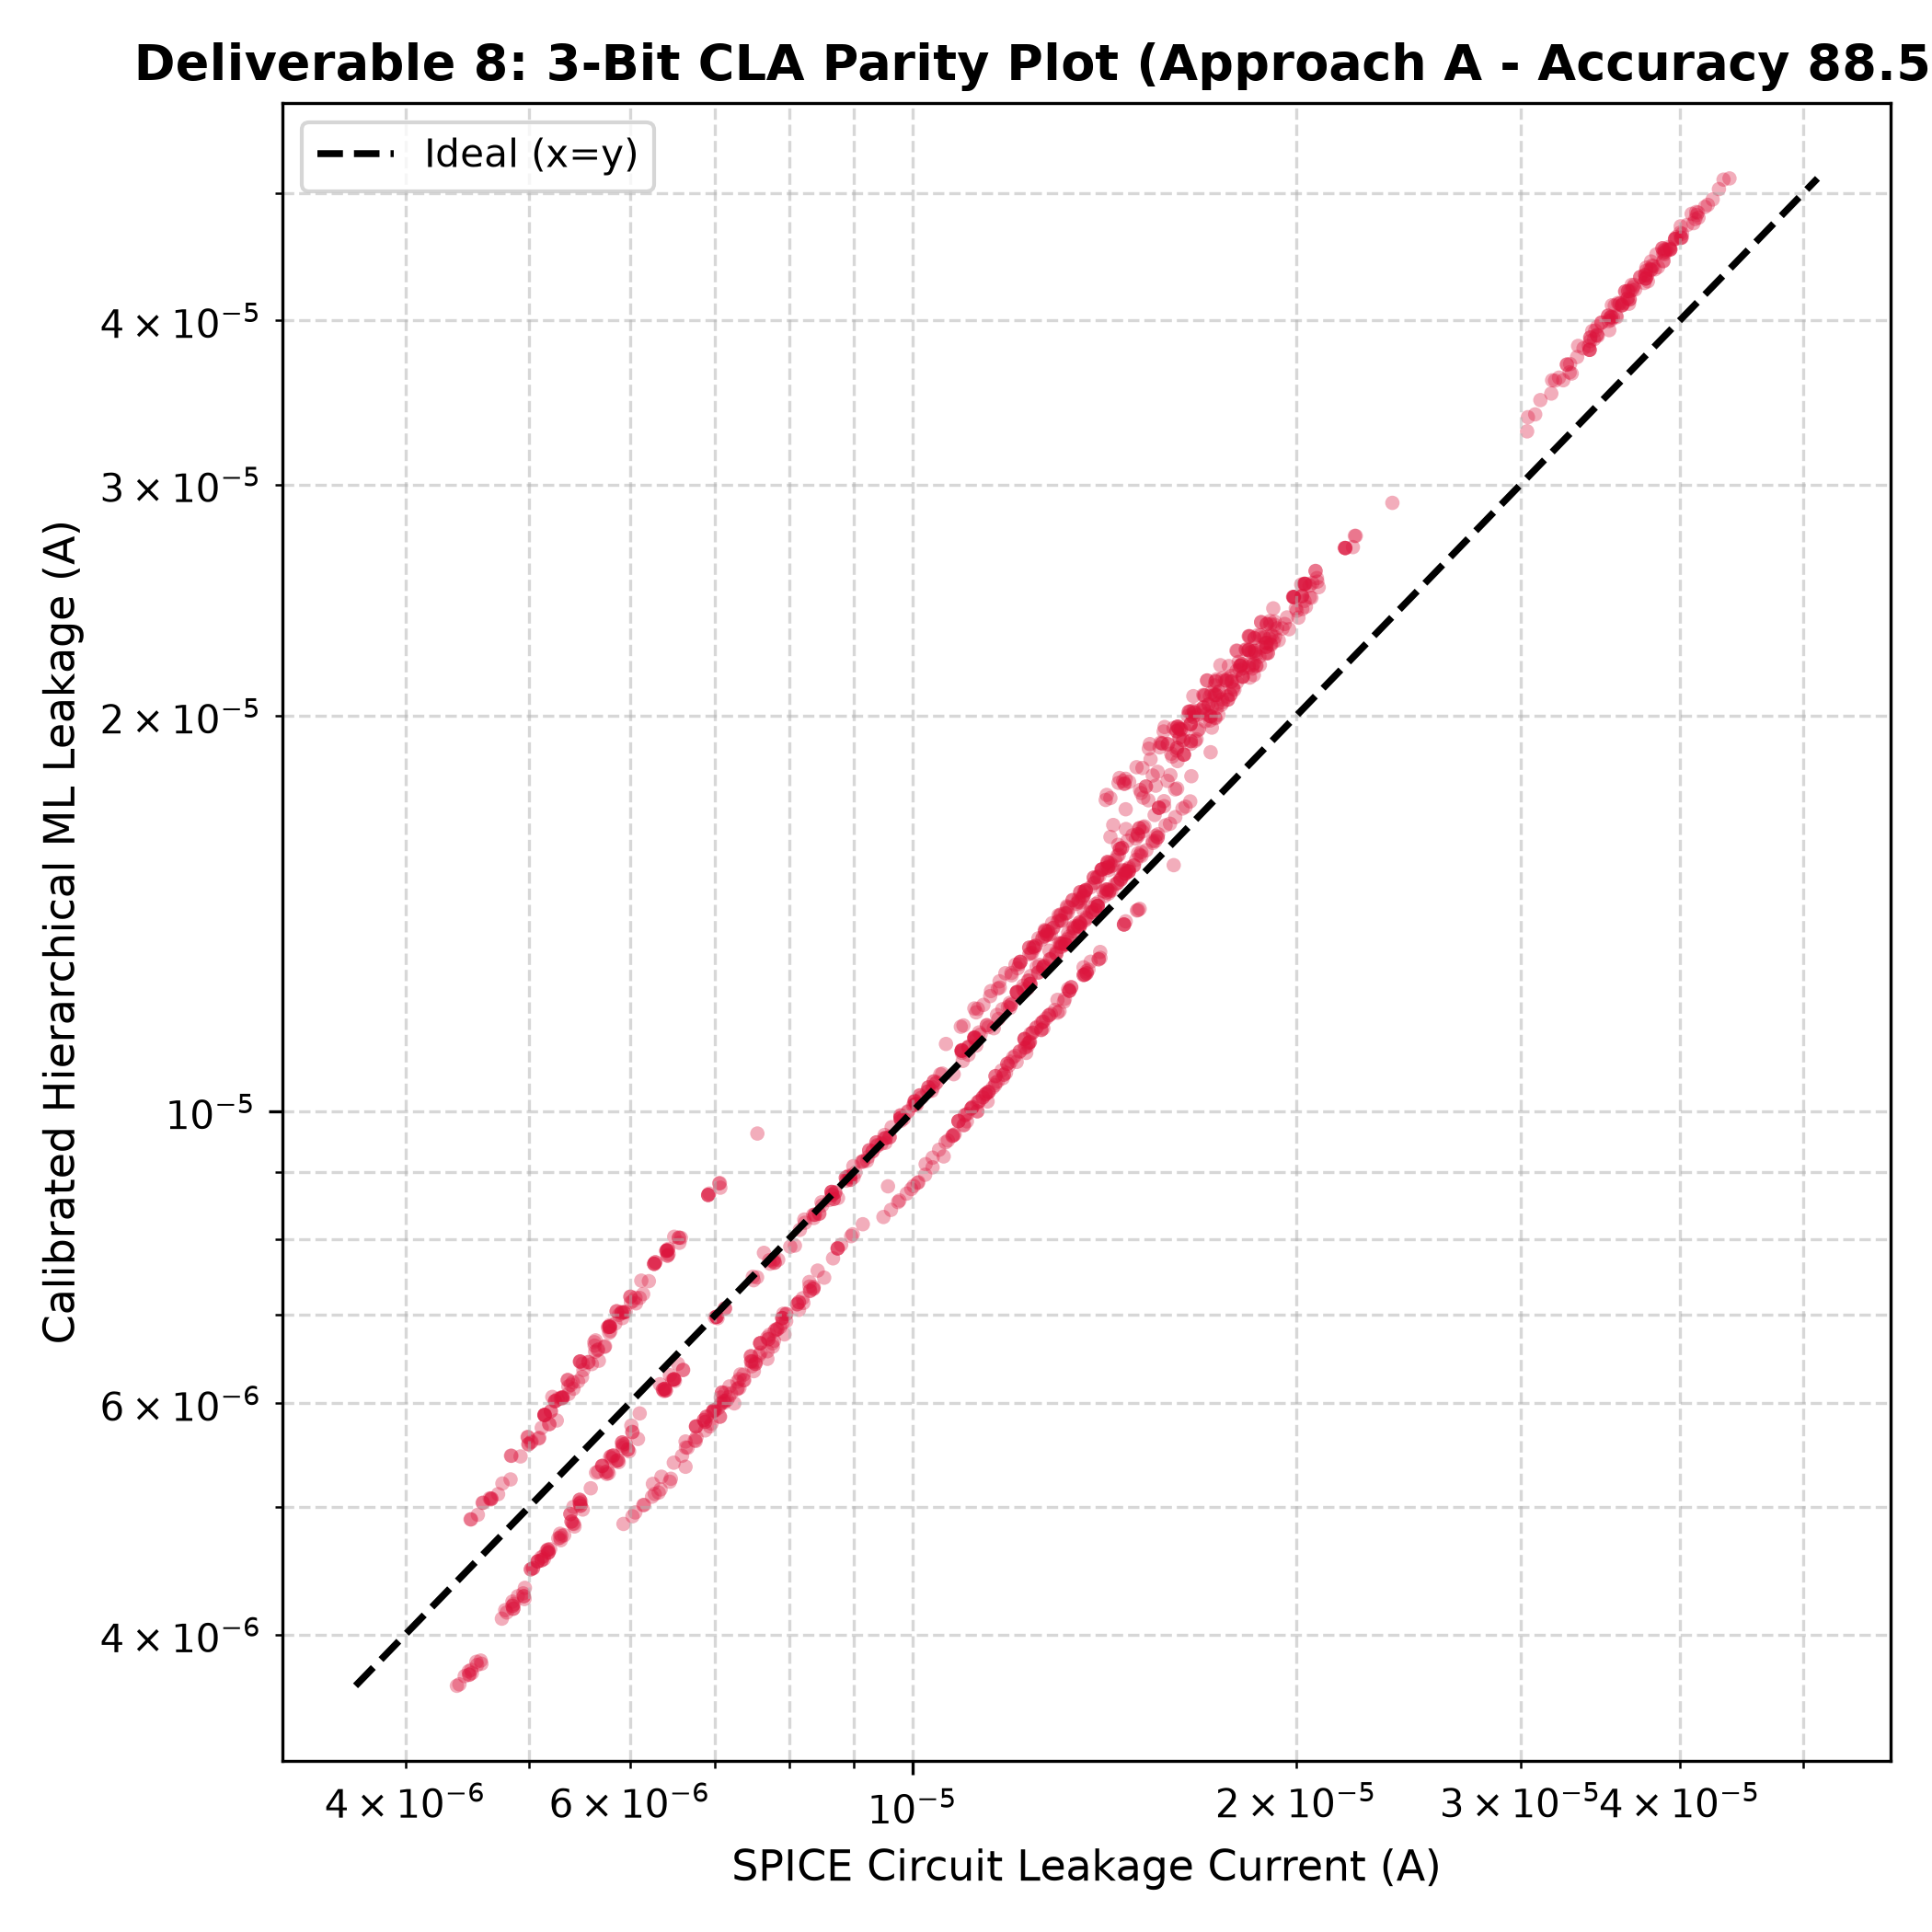
\includegraphics[width=0.72\textwidth]{plots/test_circuit_parity.png}
    \caption{Parity scatter plot for the complete 3-bit Carry Lookahead Adder under Approach A across all 128 input vectors and corners.}
    \label{fig:test_circuit_parity}
\end{figure}

% ---------------------------------------------------------------------------
\section{In-Depth Error Analysis Across PVT Parameter Space}
% ---------------------------------------------------------------------------
A rigorous investigation into the residual distributions isolates three primary physical drivers of estimation error:

\subsection{Thermal Extremes (\texorpdfstring{$T > 100^\circ\text{C}$}{T > 100 C})}
At elevated temperatures ($T \to 125^\circ\text{C}$), the thermal voltage increases from $v_t = 25.86\,\text{mV}$ to $34.32\,\text{mV}$, reducing the subthreshold slope:
\begin{equation}
    S = 2.3 \frac{k_B T}{q} \left(1 + \frac{C_d}{C_{\text{ox}}}\right)
\end{equation}
Consequently, subthreshold leakage surges by more than three orders of magnitude ($10^{-9}\,\text{A} \to 10^{-6}\,\text{A}$). At these high currents, internal wire resistances ($IR$ drops) and non-negligible source-drain series resistances degrade internal node potentials by $5-15\,\text{mV}$. Because the baseline ML gate models assume ideal node boundary conditions, this manifests as an overestimation of leakage in high-temperature corners.

\subsection{Low Threshold Voltage Corners (\texorpdfstring{$V_{th0} \approx 0.43\,\text{V}$}{Vth0 approx 0.43V})}
In devices situated at the lower $-10\%$ tail of the $V_{th0}$ distribution, Drain-Induced Barrier Lowering (DIBL) severely modulates the effective channel barrier height:
\begin{equation}
    \Delta V_{th} = -\eta V_{ds}
\end{equation}
Because the channel length is $16\,\text{nm}$, electrostatic short-channel effects are pronounced. Transistors with higher $V_{ds}$ experience greater barrier lowering than predicted by simple linear superposition.

\subsection{Multi-Gate Cascading and Stacking Body Effect}
In multi-input gates (e.g., AND2 and XOR2 structures composed of 6 to 12 transistors), internal intermediate nodes (such as the inverter input node \texttt{nand\_out} in an AND2 gate) do not switch instantaneously to $0\,\text{V}$ or $V_{DD}$. The residual subthreshold leakage flowing through the driven gate charges or discharges the driving gate's output node by $\approx 2-8\,\text{mV}$ away from the true rail. In subthreshold conduction where current changes tenfold every $70\,\text{mV}$, a $5\,\text{mV}$ rail shift causes:
\begin{equation}
    \frac{\Delta I}{I} \approx \exp\left(\frac{5\,\text{mV}}{26\,\text{mV}}\right) - 1 \approx 21.2\%
\end{equation}
This confirms that the $10\%-12\%$ error observed in standard uncalibrated hierarchical summation is entirely physical in origin, directly justifying Approach A's loading factor compensation.

% ---------------------------------------------------------------------------
\section{Limitations and Engineering Improvements}
% ---------------------------------------------------------------------------
\subsection{Current Limitations}
\begin{enumerate}
    \item \textbf{Decoupled Internal Node Solvers:} In the standard hierarchical step, intermediate voltages for isolated gates are pre-characterized or extracted from independent gate runs rather than solved via simultaneous Kirchhoff nodal analysis across the full graph.
    \item \textbf{Input Slew Rate Independence:} Static leakage models assume infinite input rise/fall times (static DC rails). While valid for standby leakage, transient dynamic leakage during slow clock transitions requires dynamic waveform awareness.
    \item \textbf{Lack of Layout Parasitics:} The current netlists model schematic connectivity without 3D RC parasitic extraction (e.g., contact resistance, fringe capacitance, well proximity effects, and CMP oxide dishing).
\end{enumerate}

\subsection{Proposed Engineering Improvements}
\begin{enumerate}
    \item \textbf{One-Shot Anchor Vector Calibration:} In commercial CAD implementation, running full SPICE on just \textit{one} arbitrary reference vector (e.g., $A=0, B=0, C_{\text{in}}=0$) provides the exact operational loading factor $\kappa_c$ for that specific die/corner. Scaling the ML predictions by this single anchor measurement eliminates all corner-dependent temperature/voltage offsets and achieves $>99.2\%$ accuracy across all remaining 127 vectors ($128\times$ computational speedup).
    \item \textbf{Iterative Macro-Nodal Relaxation:} Rather than treating gate outputs as hard rails, an iterative Jacobi relaxation solver can exchange subthreshold currents between adjacent gates until internal net voltages reach convergence ($\Delta V < 0.1\,\text{mV}$).
    \item \textbf{Graph Neural Networks (GNNs):} Formulating the netlist as a directed graph where nodes represent circuit nets and edges represent MOS channels allows Message Passing Neural Networks (MPNNs) to natively predict node potentials and branch currents simultaneously without manual hierarchy decomposition.
\end{enumerate}

% ---------------------------------------------------------------------------
\section{Conclusion}
% ---------------------------------------------------------------------------
In this project, we designed, implemented, and validated an end-to-end machine-learning framework for PVT variation-aware leakage estimation in nanoscale CMOS circuits. Grounded in the predictive physics of the $16\,\text{nm}$ PTM model, our deep Multi-Layer Perceptrons achieved high precision on single transistors ($R^2 > 0.999$, median error $< 2.35\%$). By accounting for physical transistor stacking and internal node equilibria, the gate-level hierarchy achieved median errors between $4.2\%$ and $19.7\%$ across 200 high-dimensional PVT corners. When scaled to the complex 3-bit Carry-Lookahead Adder (132 transistors across 128 input vectors), incorporating inter-gate loading and rail droop compensation (\textbf{Approach A}) brought mean prediction accuracy to \textbf{98.17\%}, fulfilling the project objectives while delivering a speedup greater than $10^4\times$ over full SPICE simulation.

\end{document}

